%!TEX root = ../thesis.tex
\chapter{DemoCut: Instructional Videos from Demonstration}
\label{chapter_democut}
% \chapter{DemoCut: Generating Concise Instructional Videos for Physical Demonstrations}

Amateur instructional videos often show a single
uninterrupted take of a recorded demonstration without any edits.
While easy to produce, such videos are often too long as they
include unnecessary or repetitive actions as well as mistakes. We introduce
DemoCut, a semi-automatic video editing system that improves the quality of amateur instructional videos for physical
tasks. DemoCut asks users to mark key moments in a recorded demonstration using a set of marker types derived from our formative study.
%
Based on these markers, the system uses audio and video analysis to automatically
organize the video into meaningful segments and apply appropriate
video editing effects.
%
To understand the effectiveness of DemoCut, we report a technical evaluation of seven video tutorials created with DemoCut. In a separate user evaluation, all eight participants successfully created a complete tutorial with a variety of video editing effects using our system.

%!TEX root = ../thesis.tex
\chapter{Introduction}
\label{chapter_introduction}

When attempting to accomplish unfamiliar, complicated tasks, people often look for tutorials to follow instructions. From performing daily tasks such as cooking and operating a machine, using software applications, to physical activities like sports and dance performance, each domain involves specific ``how-to'' knowledge with a certain degree of complexity~\cite{ryle1945knowhow}.
%
Instructions, which describe how a specific goal can be accomplished, are a tool for people to self-learn a task~\cite{Smith03iimanufacturer}. Studies have shown that visual instructions are cognitively favorable by people as they are easier to comprehend and remember than text information~\cite{Harrison:1995uh,mayer1996less,Heiser:2004:IVC:989863.989917}. In history, pictorial instructions have been created from the Middle Age to explain dancing or weapon operations~\cite{mijksenaar1999open}. It was found that the first use of letters in technical drawing for text referral was by Italian polymath Leonardo da Vinci. In 1737, French engineer de B{\'e}lidor~\cite{de1737architecture}'s diagrams were the first to apply arrows to indicate direction of movements (see Figure~\ref{fig:intro_arrows}).
%
From 1760, when the Industrial Revolution introduced mass production, instructions have been seen widely for various products and uses.

\begin{figure*}[h!]
  \centering
  \begin{minipage}{\textwidth}
  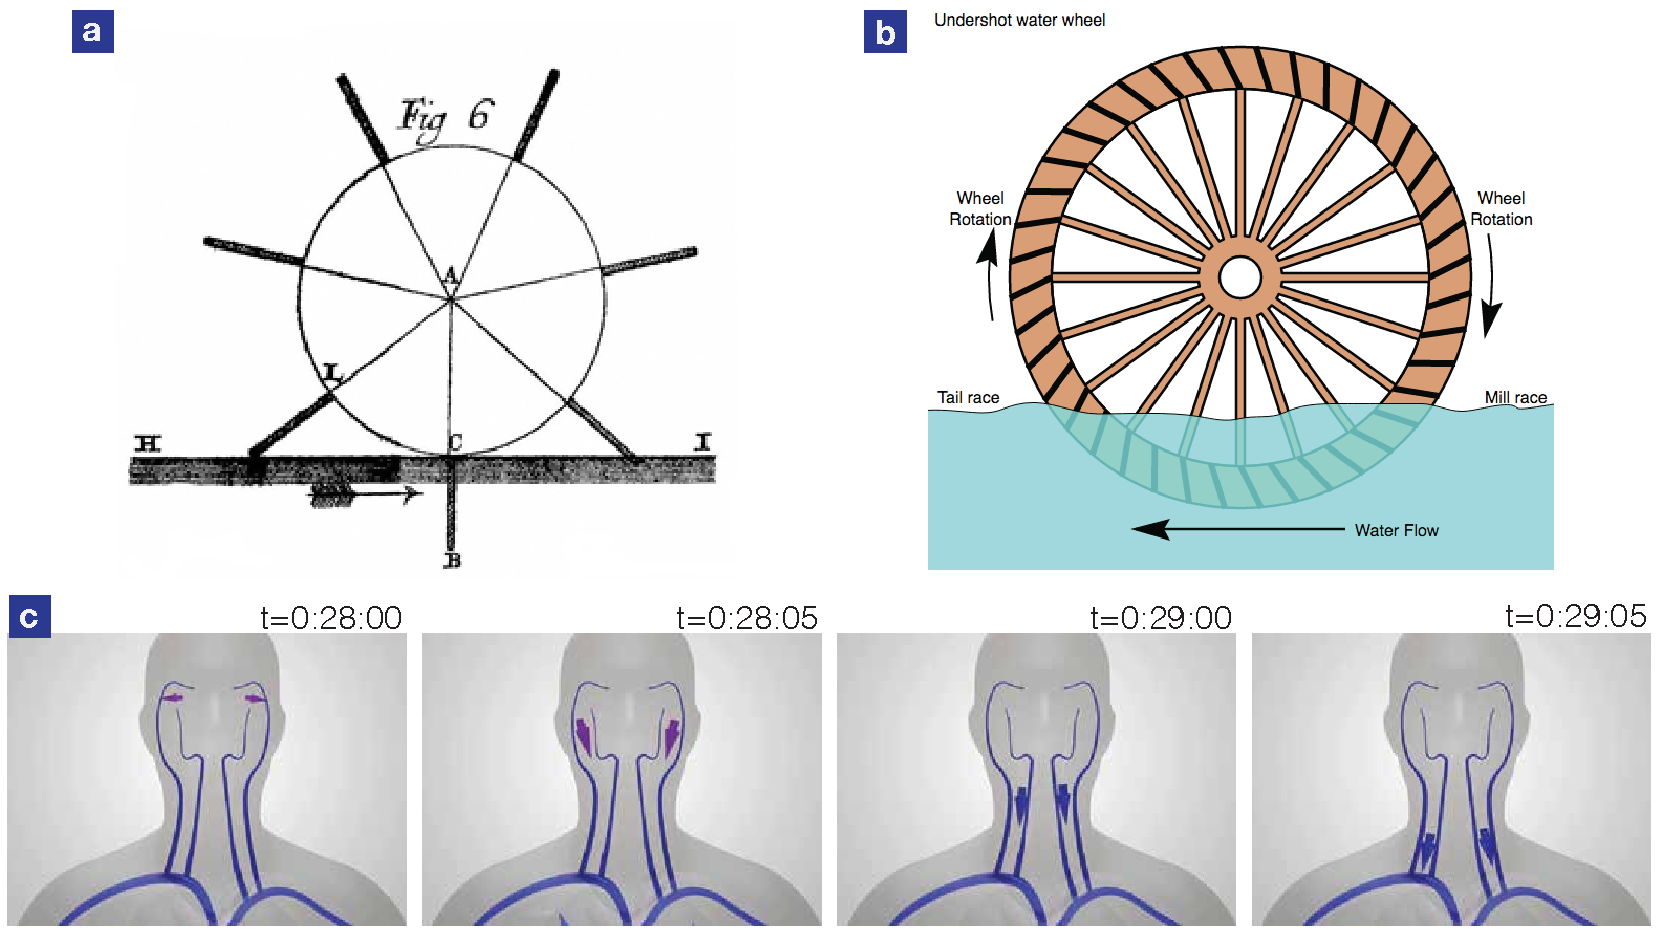
\includegraphics[width=\textwidth]{\intro/fig/arrows/arrows}
  \caption[Uses of motions arrows in visual instructions.]{Uses of motions arrows in visual instructions:
  %
  a) Year 1737: The first use of a motion arrow in an illustration explains the impact of water flow of a water wheel~\cite{de1737architecture},
  % http://www.buw-output-archiv.uni-wuppertal.de/ausgabe1/steinle/index-en.html
  %
  b) Year 2002: Similarly, arrows are used to explain the water flow and rotation of an undershot water wheel\footnote[1]{Original artwork by Daniel M. Short, ``Schematic diagram of an undershot water wheel'', licensed under CC BY-SA 2.5},
  % https://en.wikipedia.org/wiki/File:Undershot_water_wheel_schematic.svg
  %
  c) Year 2014: An animation visualizes the blood flow using motion arrows\footnote[2]{Video by Bioscience Credentials, ``Blood Flow in the Human Body'', \url{https://youtu.be/GwX41xm9esY}, licensed under CC BY 3.0}.
  }
  \label{fig:intro_arrows}
  \end{minipage}
\end{figure*}

Since the late 1990s, the advance in computer technologies has introduced more versatile instructional design. Instructions can now be created via software tools rather than hand drawing; they can include multimedia such as images and videos in several forms; they can be accessed through the Internet, as well as in hard copy.
%  the general purpose computers and the Internet
%
This advancement also enables consumers or end-users to document and share their domain knowledge~\cite{Lafreniere:2012tl}. As of today, popular tutorial sharing sites like Instructables has over 220,000 articles~\cite{InstructablesProjects}, wikiHow provides over 192,000 articles~\cite{wikiHowStatistics}, Food.com serves over 500,000 user-generated recipes with 125,000 photos~\cite{FoodComAbout}, and YouTube hosts over 285 million How-To videos\footnote{YouTube, \url{https://www.youtube.com/}, accessed June 2016}.
%
The variety of topics, content, and presentation styles provides learners more options to understand domain knowledge.
%
However, navigating a tutorial using existing tools remains inefficient for following step-by-step instructions. It can be challenging to observe details from text and images or find specific piece of information in a video through a timeline with conventional video players.
%
On the other hand, producing high-quality instructions that are easy to follow requires authoring expertise and a significant time investment. It involves several stages to design, record, and edit multimedia materials of a task using a variety of creation tools~\cite{Torrey:2007he,Tseng:2014:PVP:2598510.2598540,Muller:2009tw}.\\

The goal of this dissertation is to investigate interactive instructional design and develop computational tools that support the authoring process.
%
To contribute to computational methods of authoring user-generated instructions, two research questions that this work focuses on are:

\begin{itemize}
  \item How can authoring tools support domain experts in efficiently creating effective, high-quality instructions based on video-recorded demonstrations?
  \item How can new tutorial formats help authors better express their intent and help learners understand and follow the author's instructions?
\end{itemize}

This dissertation presents video-based computational approaches that enhance tutorial creation and consumption from author demonstrations.
We encode the current practices from professional authors into automatic algorithms and interactive techniques.
Our goal is to dramatically increase the quality of amateur-produced video instructions, which in turn improves learning for viewers who interactively navigate the content.
%
We will introduce five interactive systems that we develop to address these challenges. These tools cover both software applications (e.g., image manipulation tasks or browser navigation) and physical activities (e.g., Do-It-Yourself projects or dance movements) for recording, editing, and replaying instructional content.

% ---------------------------------------------------------------

\section{Challenges of Creating and Consuming Instructions}

Visual instructions are the dominant form of instructional design~\cite{mijksenaar1999open}. Cognitive load theory of multimedia learning suggests that learners process information using distinct channels, one for visual and the other for verbal formats~\cite{sweller1998cognitive,sweller1988cognitive,paas2003cognitive}. It was found that learners performed better when received a pictorial summary of a scientific system than those who received the full text alone or the full text with the summary~\cite{mayer1996less}.

Among all the multimedia support, videos are a common form to present instructions. We suspect that the great popularity of videos is due to the following reasons:
%
First, consumer devices and software have become affordable for authors to quickly record activities and later share via online platforms at minimum cost.
%
% ** describe the difficulties of making knowledge "explicit", esp. for actions and motions
Second, videos can be an efficient medium to document activities. Transferring know-how concisely and effectively to the audience is challenging. It especially requires efforts when a task involves \emph{tacit knowledge}, which is a kind of knowledge that is difficult to articulate in a written or verbal form~\cite{polanyi1958personal, Klemmer:2006:BMF:1142405.1142429}. Examples of tacit knowledge include dancing, riding a bike, or driving nails with a hammer. Dancers can perform movements fluently with music. If they are asked to focus on the composite pieces, such as the arm and foot actions or rhythm, they might get confused and fail to express the entire movement~\cite{polanyi1958personal}. Very often, recording a video eases the difficulties of describing the entire activities in an explicit form.
%
This leads to another motivation that videos also provide an effective channel to convey ideas with adequate amounts of details. Learners can visually observe the exact actions in a video as if an expert were coaching in person~\cite{Kuznetsov:2010:REA:1868914.1868950}.

However, while videos are easy to produce, they can include a lot of unnecessary footage. Inevitable content such as pauses, mistakes, and long repetitive actions makes it difficult for learners to focus on the most important steps and actions. A lot of authoring effort commonly goes into extracting footage, applying visual effects, and adding subtitles and annotations.
%
In addition, even with a well-edited video, navigating using a conventional video player remains inefficient. Learners with various needs could have a hard time skimming to an interesting moment or perceiving high-level overviews. Alternatively, a pictorial summary or static step-by-step tutorials presented with text and images can effectively guide knowledgeable learners through familiar tasks.

% The goal of this dissertation to develop video-based recording, editing, and playback tools are optimized for creating and consuming instructional demonstrations. I combine the advantage of ubiquitous video recording with the benefits of video and structured tutorial formats. I aim to dramatically increase the quality of amateur-produced video instructions, which in turn improves learning for viewers who interactively navigate the content.

% ----- MixT ----- %

\subsection{New Tutorial Formats}

Both static and video tutorials have strengths, but neither format alone is well suited for all learning needs that learners may have.
%
To combine the benefits, we design a new instructional presentation called \emph{MixT} (mixed-media tutorials) that improves learners' success in following instructions (see Figure~\ref{fig:mixt_intro}).
%
MixT presents step-by-step static instructions and includes in-place video clips for each operation.
%
With MixT, learners can quickly scan forward and backward on a web page to obtain an overview of a task. Embedded videos help them understand continuous, complex manipulation, such as brushing on a canvas and adjusting control points.
%
MixT's playback UI allows learners to interactively control \emph{when} to see images or videos, and \emph{how} to render videos.
%
Video editing techniques are applied to emphasize instructions, including cropping salient screen regions and highlighting interaction.
%
In our within-subject experiment, MixT successfully reduced numbers of errors and attempts made by learners when following image manipulation tasks.
% To demonstrate , MixT captures screencast video and operation events of a software demonstration.

\begin{figure*}[t]
  \centering
  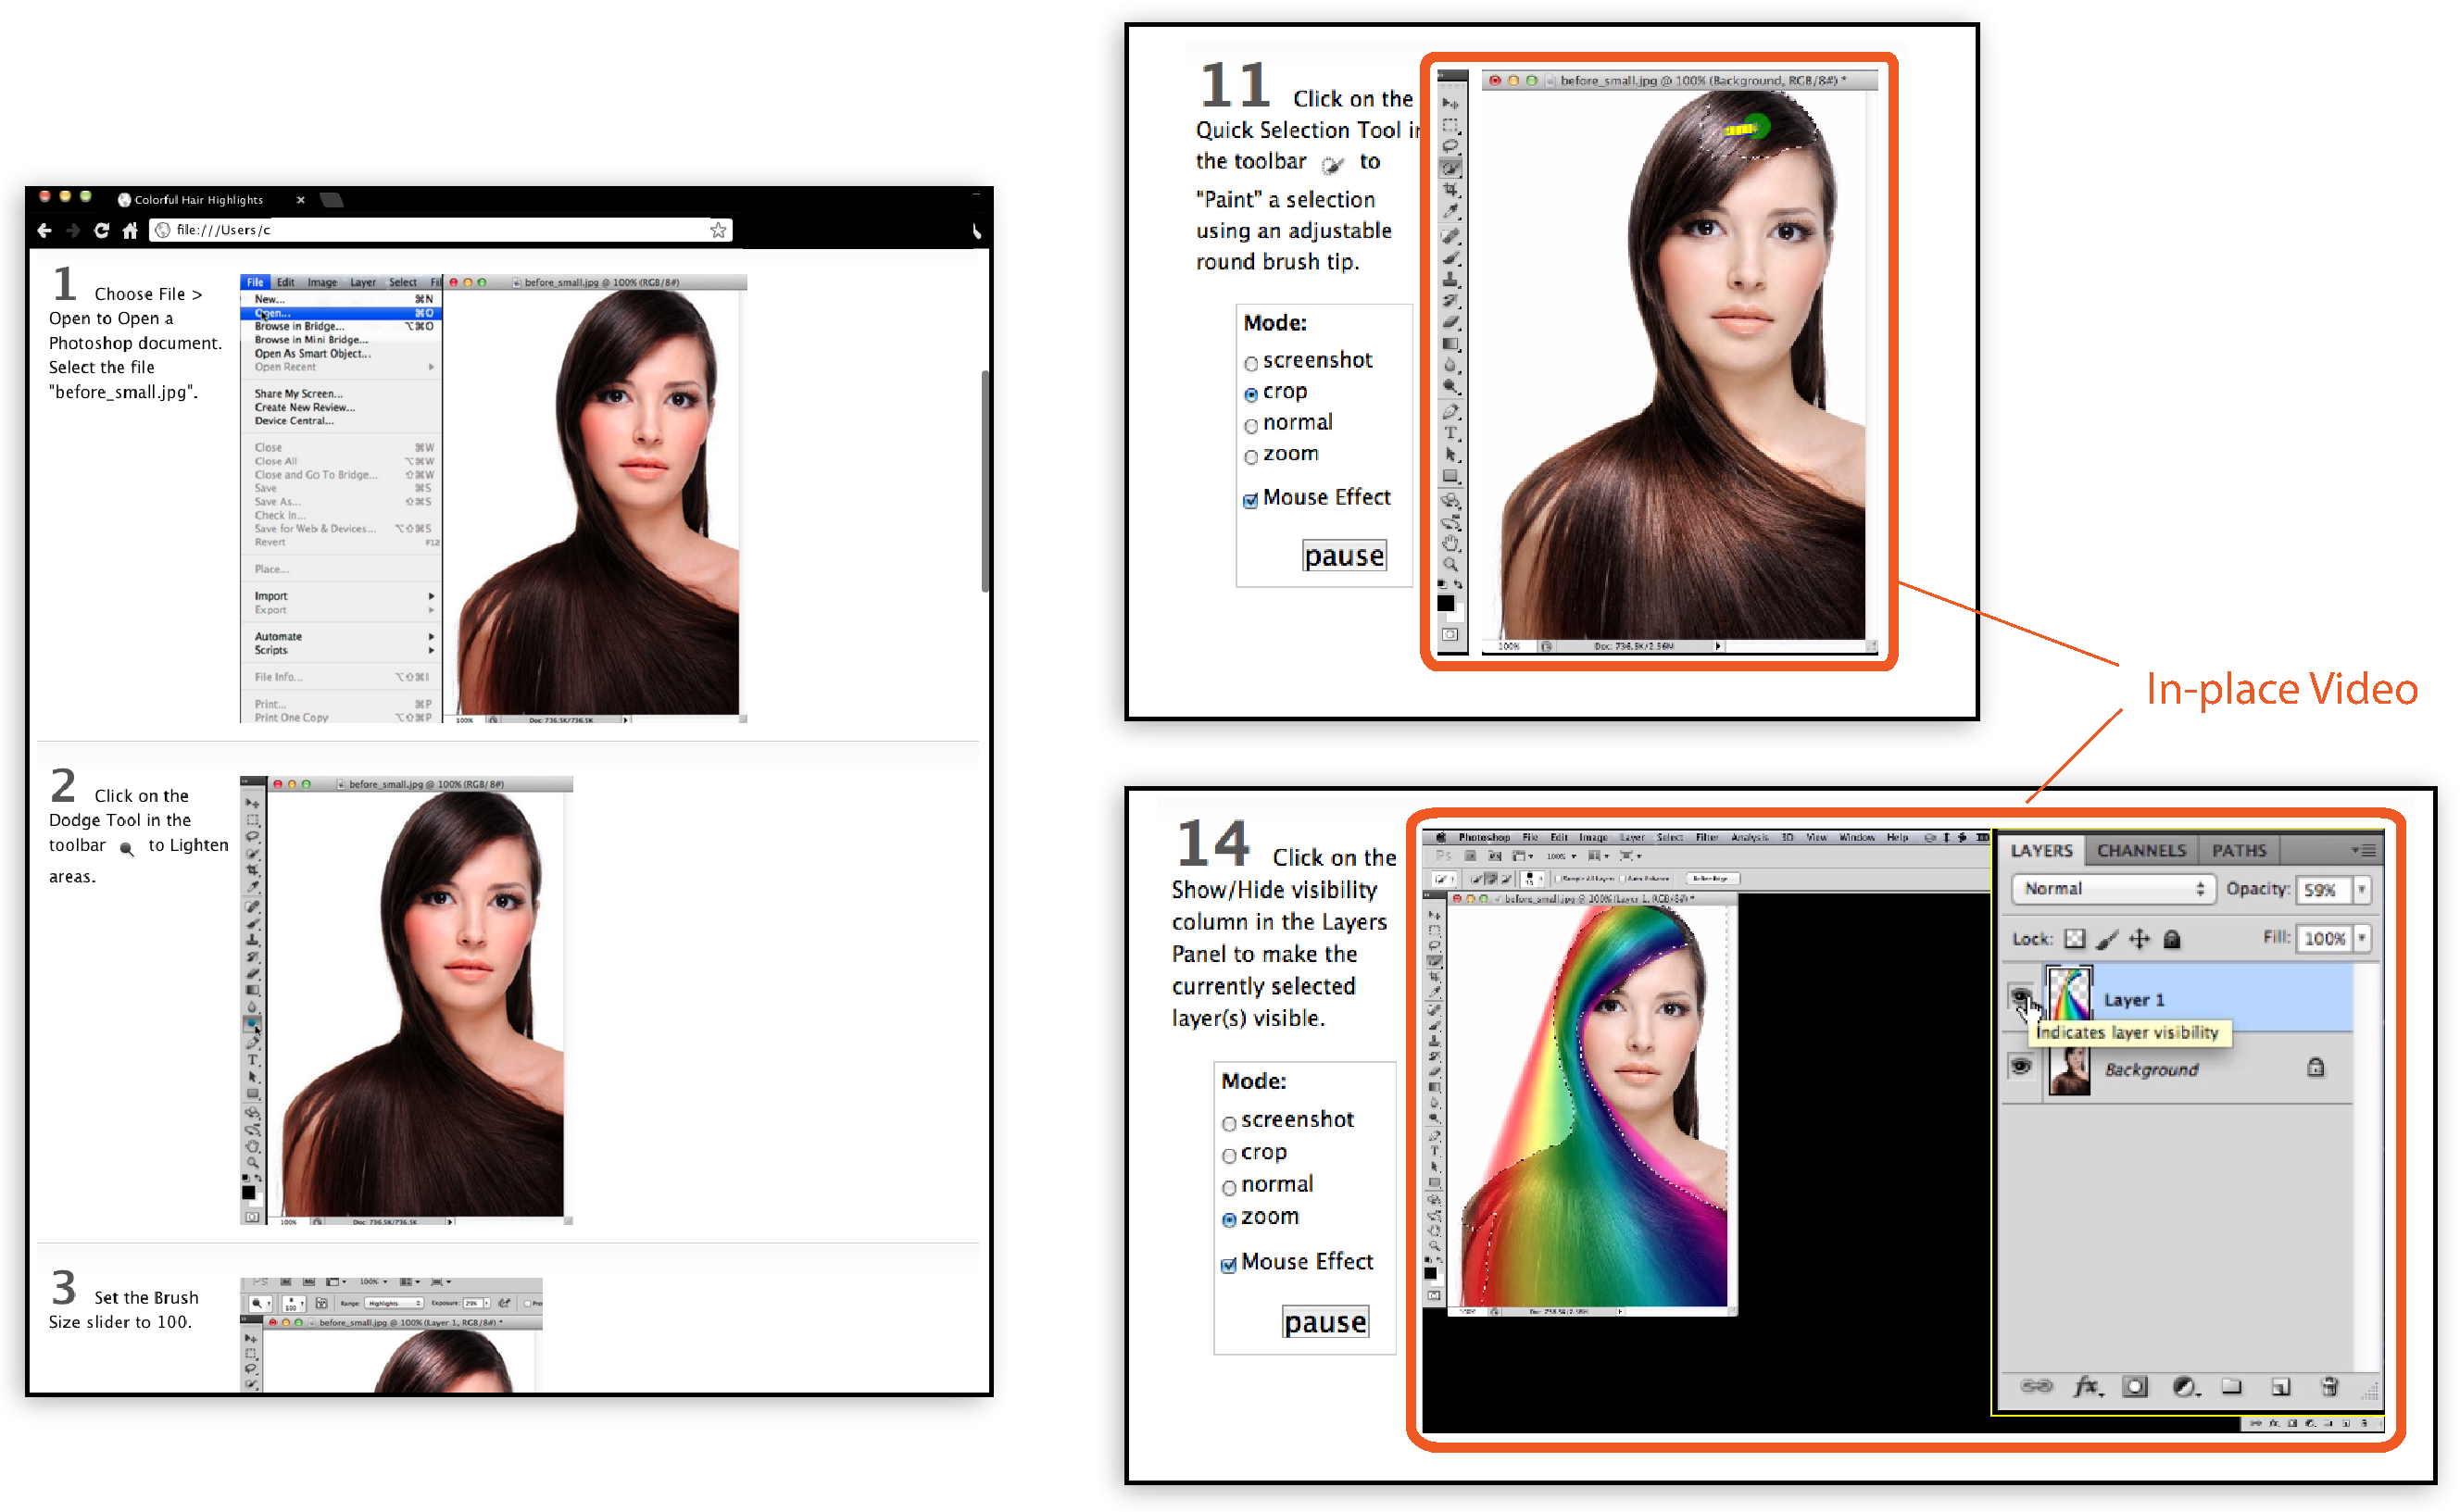
\includegraphics[width=0.8\textwidth]{\intro/fig/mixt_intro}
  \caption{MixT generates step-by-step tutorials (left) that contain static and video information from task demonstrations. Videos are automatically edited and offer different views (right) to highlight the most relevant screen areas for a step. Visualizing mouse movement helps learners understand a complex action.}
  \label{fig:mixt_intro}
\end{figure*}

% ----- DemoWiz ----- %
MixT offers a novel way of navigating instructional content with a combination of static step-by-step and embedded video presentations. If an author wants to narrate over a video recording to illustrate a demo, it can be challenging to pace oneself at the suitable timing without expecting \emph{when} and \emph{what} action is taking while a video is playing.
%
We design \emph{DemoWiz}, a system that augments a screencast video with visualizations (Figure~\ref{fig:demowiz_intro}). By logging the input events of a software demonstration, DemoWiz overlays glyphs to visually guide viewers to the next action along with the time remaining before the action occurs. This enables viewers to anticipate the video content rather than react to it.
%
Our study showed that fewer anticipation errors and narration delays were made with DemoWiz.

\begin{figure*}[t]
\centering
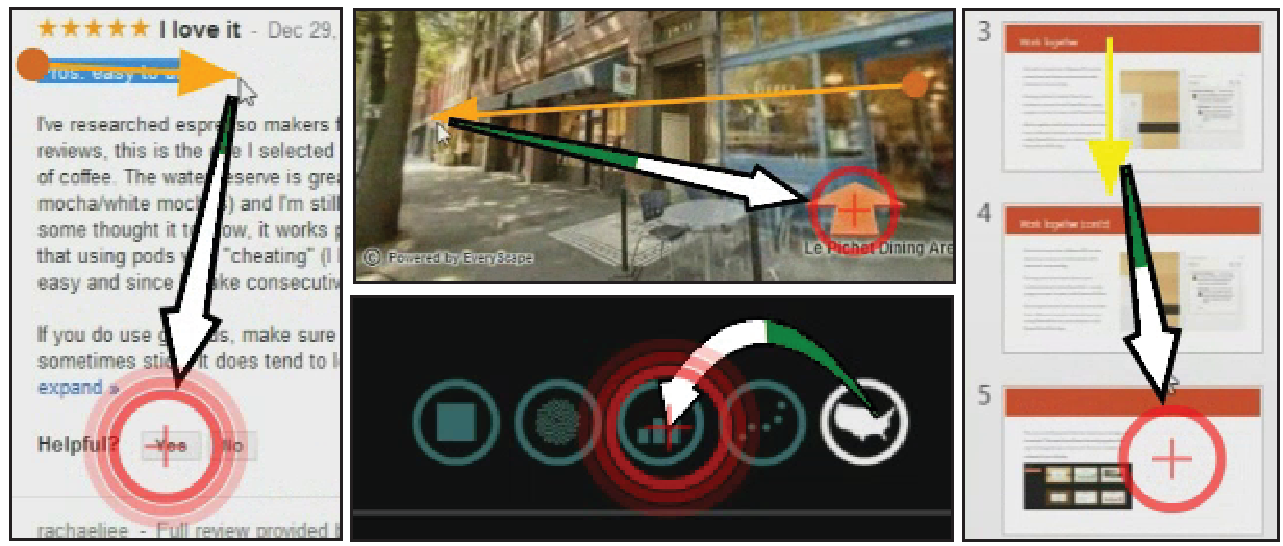
\includegraphics[width=0.7\columnwidth]{\intro/fig/DemoWiz}
\caption{DemoWiz visualizes input events in a screencast video to help viewers anticipate the upcoming event for following a software demonstration.}
\label{fig:demowiz_intro}
\end{figure*}

\subsection{Tutorial Generation from Software Demonstration}

While new tutorial formats are shown to be useful, manually creating instructions can be extremely time- and effort-consuming. In response, we design computational methods to automate the creation process from an author demonstration. MixT and DemoWiz capture screencast video and input device events from a demonstration of a task in a software application. MixT also records application commands for video analysis. Computer vision and visualization techniques are integrated to segment a video into steps, extract salient information, and add visual highlights.
%
In addition, DemoWiz supports an editing phase where authors can adjust the timing of events in a video. Playback speed of recorded actions can be modified or skipped via an editing UI. Our studies showed that our algorithms for step segmentation, event detection, and visualization were effective (\textless8\% error rate in MixT and 0\% in DemoWiz).

\subsection{Interactive Tutorial Authoring from Physical Demonstration}

% ----- DemoCut ----- %

Moving beyond software applications, support for authoring instructions of tasks that take place in the physical world is lacking. Activity recognition remains an open research question, and making authoring decisions during a demonstration can be difficult.
%
To address this problem, we first look into Do it yourself (DIY) project tutorials, which help people learn knowledge and skills to complete a task independently.
%
We developed \emph{DemoCut}, a semi-automatic video editing system that improves the quality of amateur instructional videos for physical tasks (Figure~\ref{fig:democut_intro}). DemoCut asks authors to describe key ``moments'' in a recorded demonstration video using a set of markers. Based on the annotations, our system analyzes the audio and visual activities to automatically organize the video into meaningful segments. Editing decisions are applied to support both \emph{temporal effects} that increase playback speed or skip segments, as well as \emph{visual effects}, such as zooming, subtitles, and visual highlights. A playback interface allows authors to quickly review and edit the automatically generated effects.
%
Our studies showed that video tutorials created by DemoCut in five DIY domains were concise in terms of video length and descriptive instructions with low effect error rates.

\begin{figure*}[t]
  \centering
  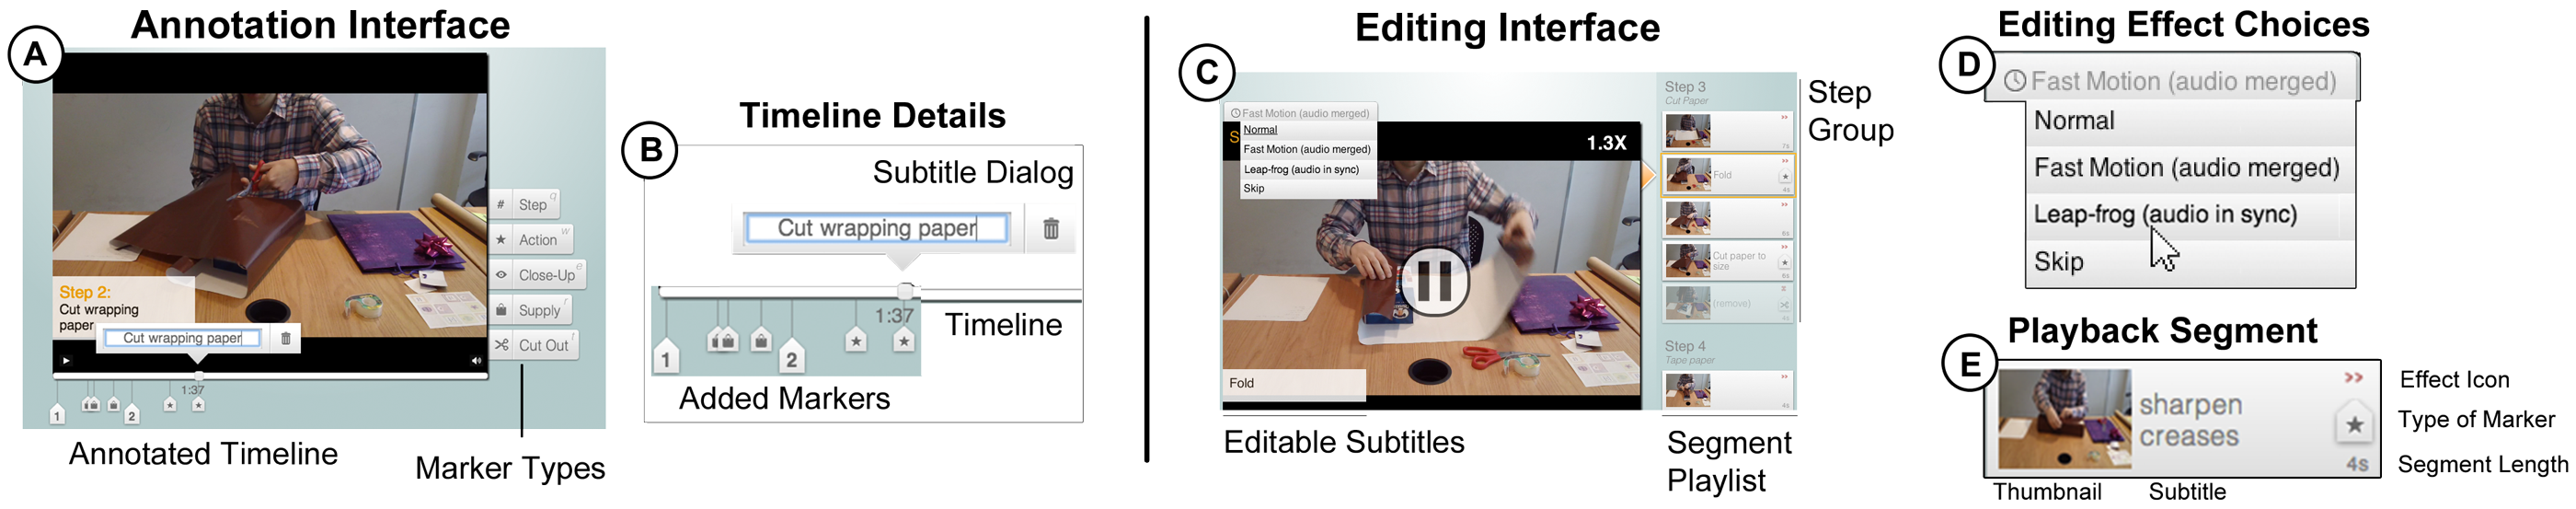
\includegraphics[width=\textwidth]{\intro/fig/DemoCut}
  \caption{DemoCut asks authors to mark key moments in a recorded video of demonstration using a set of marker types. Based on marker information, the system uses audio and video analysis to automatically organize the video into meaningful segments and apply appropriate video editing effects, which can be modified via a playback UI.}
  \label{fig:democut_intro}
\end{figure*}

% ----- Kinectograph ----- %
Through the process of designing DemoCut for automatic DIY video editing, we observed that for tasks that require larger space and more movements, instructors often have to adjust the position and viewing angle of a camcorder. Some authors choose to set up multiple cameras and later select the best shot from video streams, while some invite another person who controls the camcorder during a demonstration.
%
To enable authors to record their demonstration without acquiring additional cameras or cameraman, we design \emph{Kinectograph}, a video recording device with a single camera that automatically tracks and follows specific body parts, e.g., hands, of an instructor in a video (see Figure~\ref{fig:kinectograph_intro}). It utilizes a Kinect depth sensor to track skeletal data and adjusts the camera angle via a 2D pan-tilt gimbal mount. Authors can freely move around in space to demonstrate a task and monitor real-time video preview through a tablet application.

\begin{figure}[!t]
  \centering
  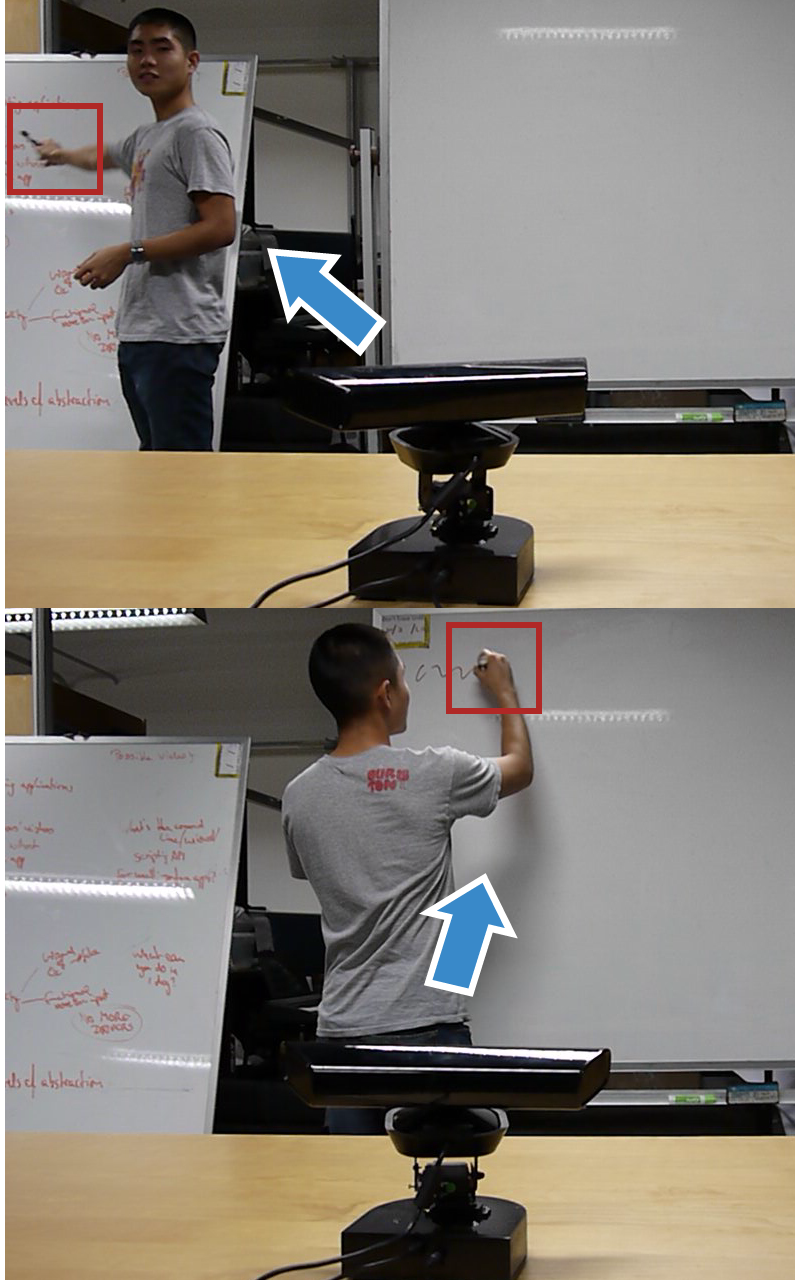
\includegraphics[width=0.65\columnwidth]{\intro/fig/Kinectograph}
  \caption{Composed of a Kinect camera to track author movement and a motorized dock to pan and tilt the camera, Kinectograph allows the author (or their hand) remains centered in the recorded video in real-time.}
\label{fig:kinectograph_intro}
\end{figure}

% ----- DemoDraw ----- %

The successful experiences supporting motion-based recordings motivated me to apply our demonstration-based approach to a domain that is entirely driven by movements. In sports, dance performance, and body gesture interfaces, movement instructions are often conveyed with drawings of the human body annotated with arrows or stroboscopic effects~\cite{cutting_representing_2002}. However, current practices require authors to manually sketch or trace subjects from photographs, which is time-consuming and difficult to make changes once created.
%
We design \emph{DemoDraw}, a system that generates concise illustrations from author demonstration (see Figure~\ref{fig:demodraw_intro}). With DemoDraw, an author records one or more motions by physically demonstrating in front of a Kinect sensor. In a multi-modal Demonstration Interface, DemoDraw segments speech and 3D joint motion into a sequence of motion segments, each characterized by a key pose and salient joint trajectories. Based on this sequence, a series of illustrations is automatically generated using a stylistically rendered 3D avatar annotated with arrows to convey movements. Once a suitable sequence of steps has been created, a Refinement Interface enables fine control of visualization parameters.
%
In a three-part evaluation, our results show 4 to 7-step illustrations can be efficiently created in 5 or 10 minutes on average.

\begin{figure}[t]
  \centering
  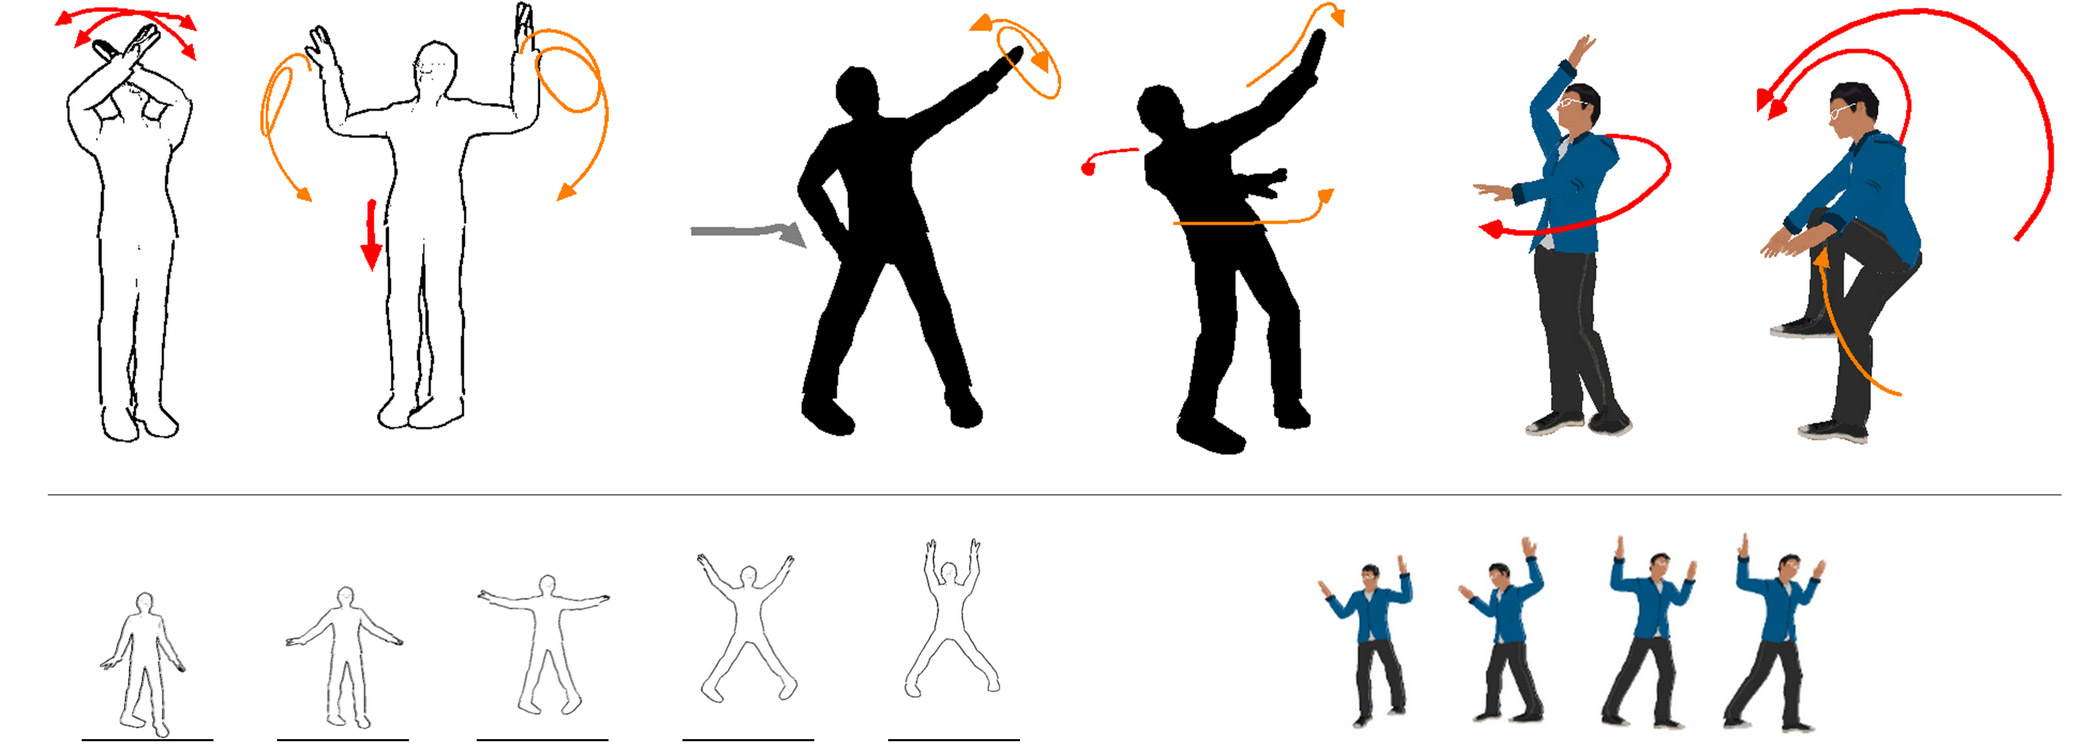
\includegraphics[width=\columnwidth]{\intro/fig/DemoDraw}
  \caption{DemoDraw's multi-modal approach enables authors to capture motion, verify results, and re-perform portions if needed to generate step-by-step motion illustrations.}
  \label{fig:demodraw_intro}
\end{figure}

% ---------------------------------------------------------------

\section{Thesis Contributions}

Overall, our video-based approaches consider key events or moments that are important to a learner. This information can be derived from software event logs or human annotation of physical tasks when automatic recognition remains challenging. Based on the metadata and video streams, we propose automatic methods to generate concise instructions for two task domains, software applications and physical tasks (see Figure~\ref{fig:space}). Our approaches support authors from recording demonstrations to editing and reviewing system-generated instructions. Interactive controls are available in different stages via desktop or multi-modal interfaces.
%
We demonstrate a series of systems that consider production stages of tutorial creation and learning. We present the rationale and technical challenges of these interactive system designs. Each system is evaluated both quantitatively and qualitatively to study the usability in authoring and learning.

\clearpage
The contributions of this dissertation include:

\begin{itemize}
\item New instructional formats that consider the learning needs from several domains, including software applications and physical activities.
\item Multi-modal interaction techniques for novice or amateur authors to create effective instructions by demonstration.
\item Automatic or semi-automatic approaches using video and audio analysis that includes authors in the loop to produce high-quality instructions.
\end{itemize}

\begin{figure}[t!]
  \centering
  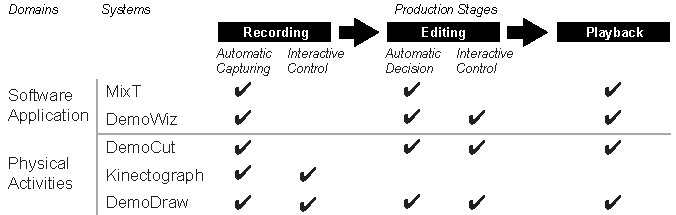
\includegraphics[width=0.9\columnwidth]{\intro/fig/space}
  \caption{A design space of the creation and consumption process for tutorials. It involves three phases of recording, editing, and playback in either software domain or a physical world. This dissertation proposes a series of systems that focus on various aspects in this design space.}
  \label{fig:space}
\end{figure}

% ---------------------------------------------------------------

\section{Overview}

The rest of this dissertation is structured as follows:
%
In Chapter \ref{chapter_background}, we define terminology used in instruction creation and consumption process based on literature. We review studies on why people rely on tutorials in general, how the formats of instructions matter, and the current practices of authoring instructions.
%
In Chapter \ref{chapter_related_work}, we review the literature on research and technologies used in supporting activities of authoring and consuming instructions.

We presented two systems that generate interactive tutorials for software applications.
% MixT
In Chapter \ref{chapter_mixt}, we present our study on how a new tutorial format supports learners in following step-by-step instructions with mixed media, including static text, images, and video clips. We introduce our creation tool called MixT, which automatically generates such new tutorial format from a software demonstration.
% DemoWiz
Chapter \ref{chapter_demowiz} introduces DemoWiz, a system that assists viewers in capturing the timing of input events in a screencast demo video. DemoWiz supports recording, editing, and reviewing stages in a production process with an authoring and playback UI.

Then, we introduced three systems designed for real-world tasks that involve physical demonstrations.
% DemoCut
In Chapter \ref{chapter_democut}, we present a semi-automatic tool for DIY video editing. Our system, called DemoCut, provides two authoring interfaces, annotation and editing, that enable authors to mark a demo video and review and modify the automatically edited results. The design is based on an fundamental understanding of DIY activities.
% Kinectograph
In Chapter \ref{chapter_kinectograph}, we focus on a recording device that automatically follows a demonstrator for filming instructional videos. The Kinectograph system tracks an author's position and body parts and provides an authoring interface for real-time camera control.
% DemoDraw
Finally, in Chapter \ref{chapter_demodraw}, we introduce a multi-modal approach for authors to generate motion illustrations by physically demonstrating the movements. DemoDraw is a system that segments speech and 3D joint motion into a sequence of motion segments and renders effective illustrations. Two authoring interfaces enable authors to navigate, re-perform, and edit visualization parameters.

% Conclusion
Throughout this dissertation, we discuss how our video-based approaches increase the quality of amateur-produced video instructions. Chapter \ref{chapter_conclusion} concludes our work on tutorial creation and consumption in both software and physical instructions. New directions for future research on interactive tutorials are proposed.

% ---------------------------------------------------------------

\section {Prior Publications}

This dissertation is based on papers published in previous ACM conference proceedings: the MixT system was published at UIST 2012~\cite{Chi:2012:MAG:2380116.2380130}, DemoWiz at CHI 2014~\cite{Chi:2014:DRS:2556288.2557254}, DemoCut at UIST 2013~\cite{Chi:2013:DGC:2501988.2502052}, and Kinectograph at CHI 2013~\cite{Cheng:2013:BCC:2468356.2468568}; DemoDraw will be published at UIST 2016~\cite{Chi:2016:DemoDraw}.

While I am primary author on all publications and led the described projects, this research could not have been completed without my advisor Bj\"orn Hartmann and my collaborators that I have been fortunately to work with. Specifically, Dr. Mira Dontcheva and Dr. Wilmot Li at Adobe Research provided valuable guidance on three projects (MixT, DemoCut, and DemoDraw); Dr. Steven M. Drucker and Dr. Bongshin Lee at Microsoft Research guided the DemoWiz project with their expertise on visualization; Professor Daniel Vogel at University of Waterloo greatly contributed to the DemoDraw project. A group of MS and undergrad students at UC Berkeley and Adobe contributed to implementation, design, and user study in the projects, including Sally Ahn and Amanda Ren in MixT, Joyce Liu and Jason Linder in DemoCut, and Derrick Cheng and Taeil Kwak in Kinectograph.

% We are all natural performers. Humans are proficient at demonstrating how to perform a task in action. However, articulating knowledge into a written or structured form can be extremely difficult. From dancing, repairing a machine, to operating software applications, it remains a challenge how everyday activities can be efficiently captured for a remote learner to understand.

%!TEX root = ../thesis.tex

\chapter{Related Work}
\label{chapter_related_work}

While existing practices require tutorial authors to create instructions manually, HCI and Computer Graphics communities have introduced novel technologies for authoring tutorials, including automatic generation methods and interactive editing tools.
%
In this chapter, I survey state-of-the-art techniques for generating instructions for both software applications (Section \ref{related_software}) and physical tasks (Section \ref{related_physical}).
%
Furthermore, existing instructions are mainly offered in the forms of conventional media, such as static tutorials (print-outs or web) or videos. With software systems, \keyword{interactive tutorials} have been introduced for learners to interactively review instructional content. I will discuss various forms of such kind of instructions by prior research, which leads to a discussion on the remaining gaps in tool support for creating and navigating instructional content.

% -------------------------------------------

\section{Instructions for Software Applications}
\label{related_software}

\subsection{Workflow Capturing and Tutorials}

Revealing operation history has shown to be effective in presenting software instructions. Operational events can range from low-level, application agnostic input device events (e.g., mouse actions, cursor movements, or keyboard strokes) to higher level, application-dependent information (e.g., menu selections or UI component changes).
%
Researchers have investigated automatic approaches that capture and visualize these types of events. Nakamura and Igarashi~\cite{Nakamura:2008:ASV:1449715.1449721} proposed a capturing and rendering system independent to GUI applications. Their system logs mouse events of a software demonstration process, including mouse moving, dragging, and clicking. Operations are rendered as markers and arrows on screenshot images to present the linear event history (see Figure~\ref{fig:related_events} top).
%
Grabler \ea{}'s approach~\cite{Grabler:2009jj} further analyzes the application context, including facial features and outdoor scenes, and annotates software screenshots with arrows, bounding boxes, and call-outs (see Figure~\ref{fig:related_events} bottom). In addition to annotated images, their system generates textual description from templates, such as \iquote{Select the \textbf{path tool} from the \textbf{toolbar} to \textbf{create and edit paths}.} The generated text and rendered images of operations are presented as a step-by-step tutorial, which is currently available as a Photoshop plug-in\footnote{Adobe labs. Tutorial Builder. \url{http://labs.adobe.com/technologies/tutorialbuilder/}}.

Demonstration-based approaches for generating instructions have been also applied to applications that involve more complicated manipulations or gestures, including 3D mesh construction~\cite{Denning:2011fy} and mobile apps~\cite{Wang:2014:EAC:2556288.2557407}.
%
Beyond logging events from recording a user demonstration, researchers have shown that workflows and software content can be captured automatically using application logs \cite{Grossman:2010jz,Grabler:2009jj,Pongnumkul:2011ju} or computer vision from analyzing desktop regions~\cite{Yeh:2009dh,Chang:2011vd} and existing screencast videos~\cite{Banovic:2012kd}.

\begin{figure*}[t!]
  \centering
  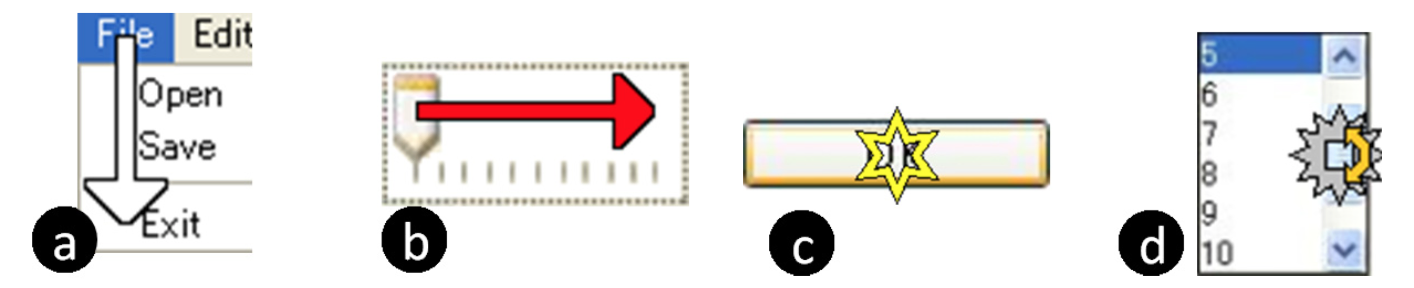
\includegraphics[width=0.6\textwidth]{\background/fig/software_viz/Nakamura_and_Igarashi}
  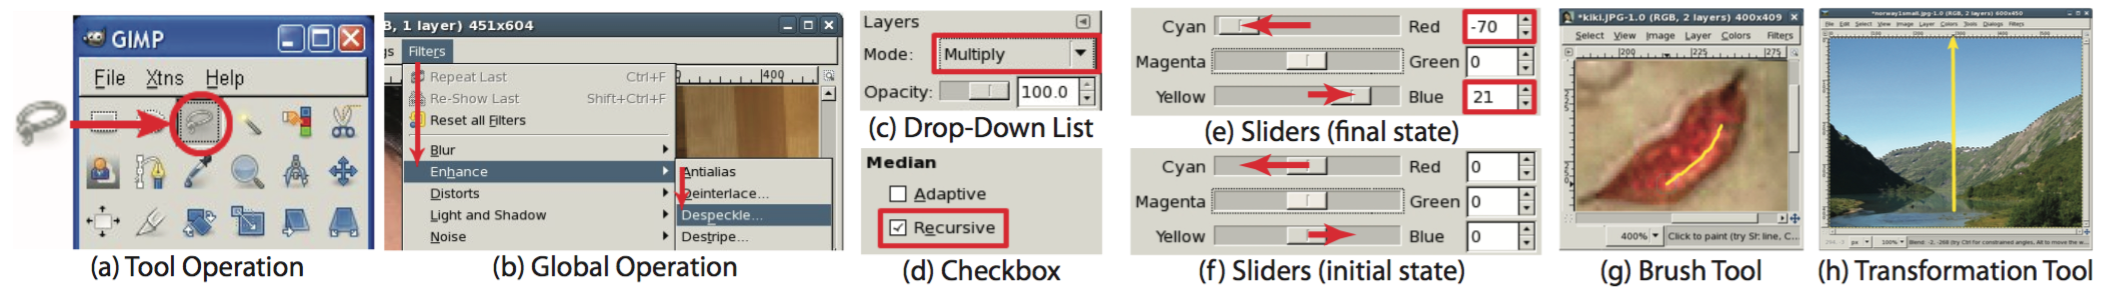
\includegraphics[width=\textwidth]{\background/fig/software_viz/Grabler}
  \caption{Example screenshots that visualize mouse operations are automatically rendered, including (top) mouse move, drag, click, and wheel (a-d) by Nakamura and Igarashi~\cite{Nakamura:2008:ASV:1449715.1449721} and (bottom) application-specific operations (a-b), parameters (c-f), and manipulations (g-h) by Grabler \ea{}~\cite{Grabler:2009jj}.}
  \label{fig:related_events}
\end{figure*}

To compare operation effects and workflows, other effective visualization approaches include showing a list of ``before'' and ``after'' thumbnails, video clips, and event timeline \cite{Grossman:2010jz} and creating a union graph of operations \cite{Kong:2012:DTR:2207676.2208549} (see Figure~\ref{fig:related_comparison}).

\begin{figure*}[t!]
  \centering
  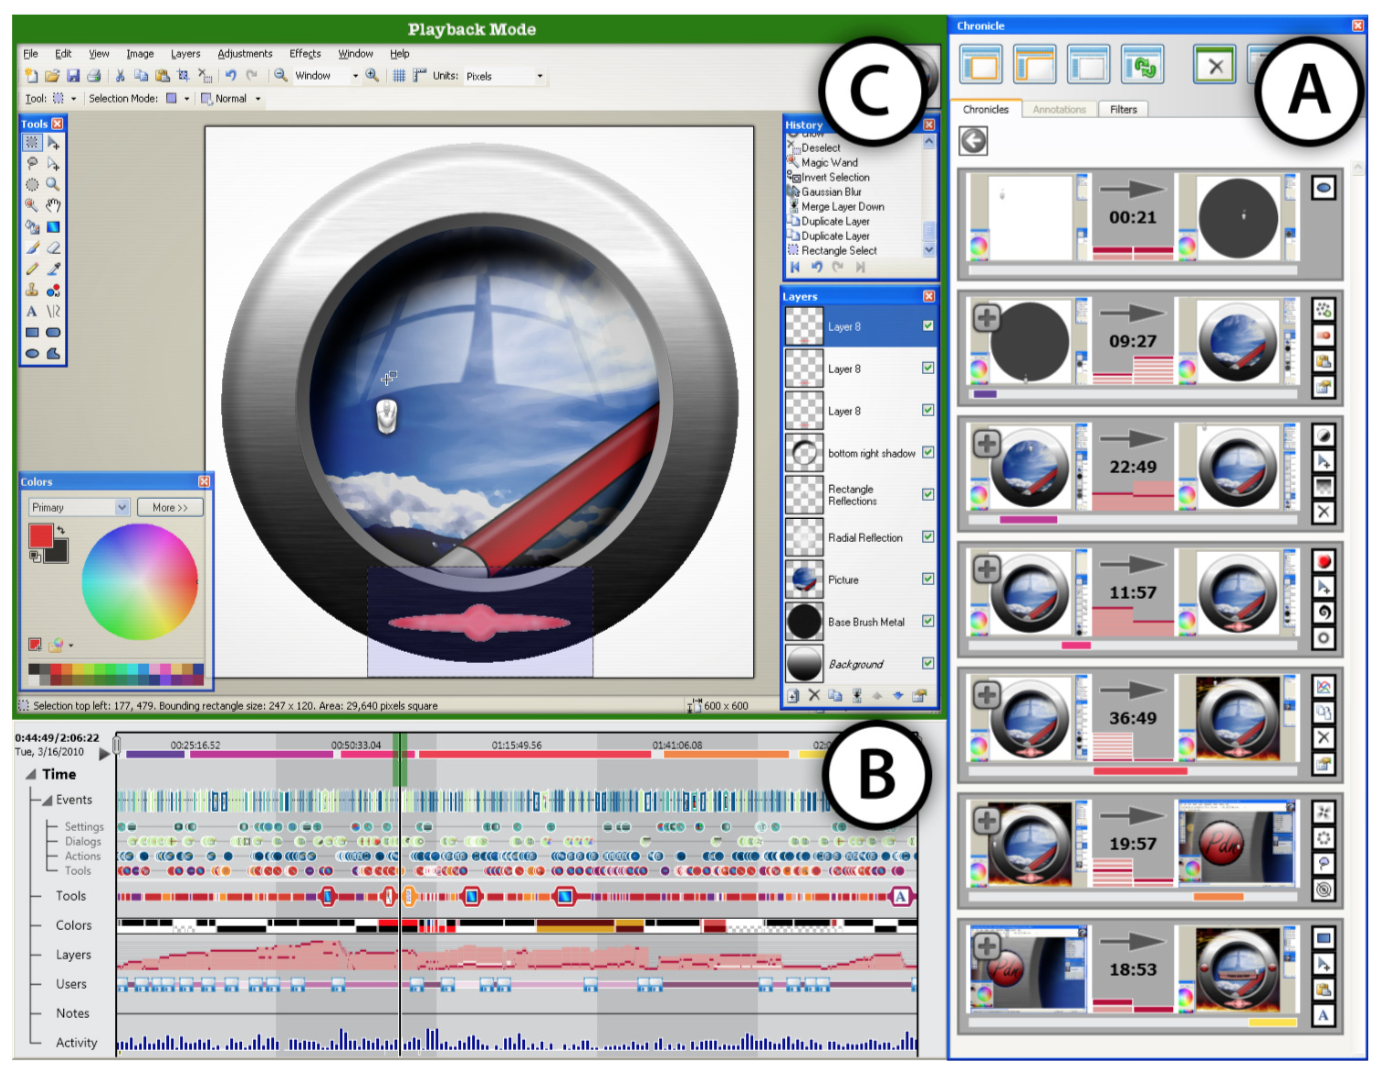
\includegraphics[width=0.4\textwidth]{\background/fig/software_viz/Grossman}
  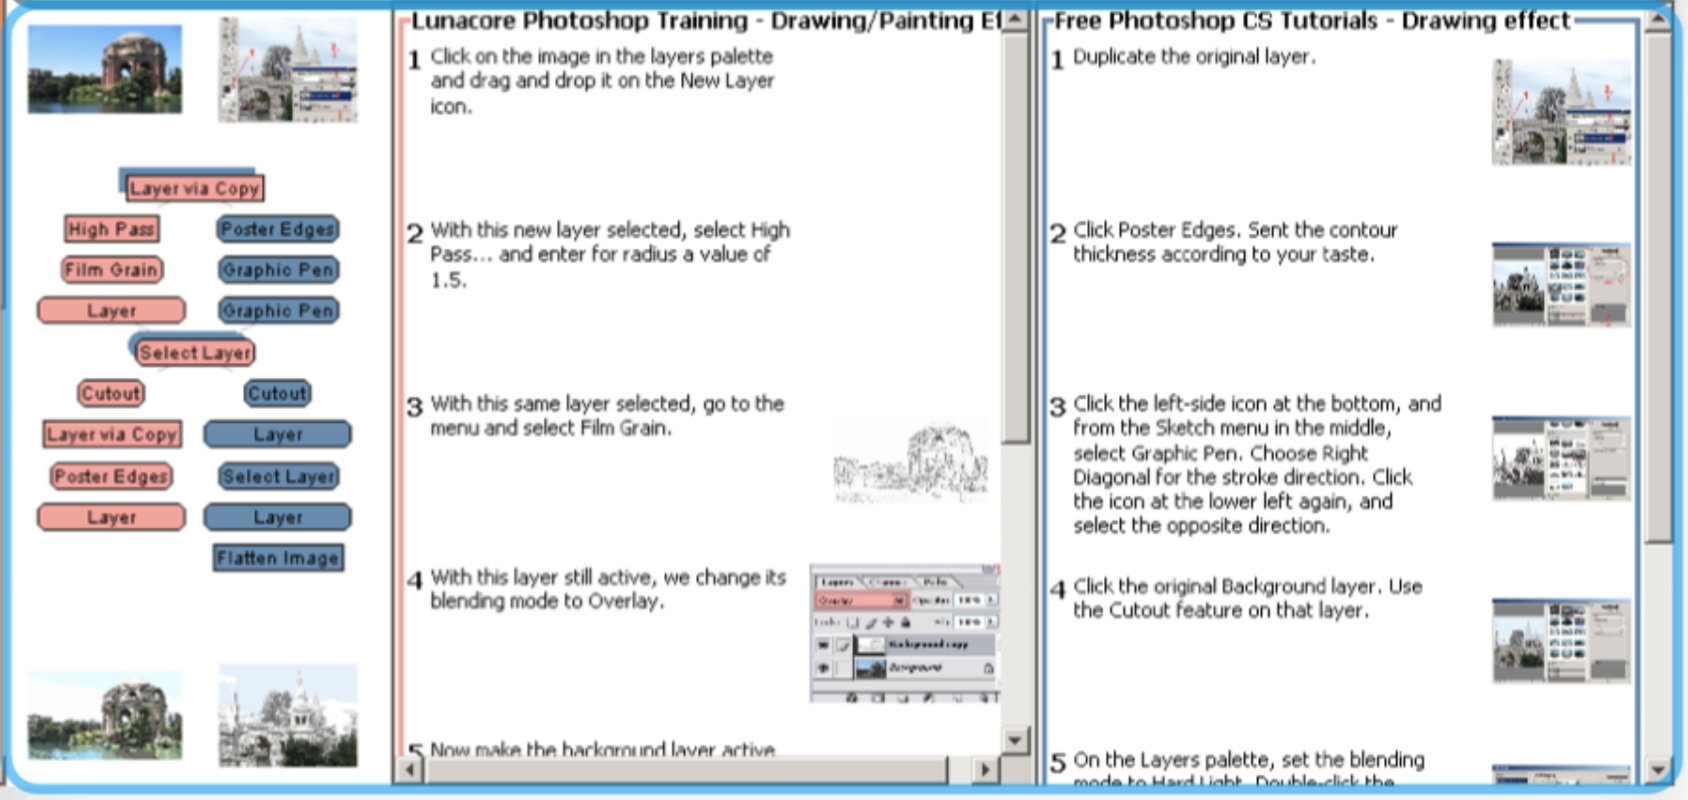
\includegraphics[width=0.55\textwidth]{\background/fig/software_viz/Kong}
  \caption{Instructional systems that help learners compare effects and similar tutorials using: (left) before and after images (a) and event timeline (b) by Grossman \ea{}~\cite{Grossman:2010jz} and (right) operation union graph by Kong \ea{}~\cite{Kong:2012:DTR:2207676.2208549}.}
  \label{fig:related_comparison}
\end{figure*}

% -------------------

\subsection{In-Application Support}

The above systems introduce innovative ways of providing informative screenshots or representations for learners to review workflows. However, reviewing these materials is often separated from operating a software application. Learners might have to switch between context of interacting an application and reading instructions, which could introduce a gap of evaluation (\iquote{Am I doing this right as the instructions explain?}) and a gap of execution (\iquote{How do I perform the action that the instructions describe?}).
%
Researchers have proposed another approach to provide ``in-application'' assistance, often in real-time, in a specific application context.

Studies have shown that visualizing input events in real-time during operations can provide better learnability of applications \cite{Dixon:2010fb}.
%
Commercial tools such as Mouseposé\footnote{Mouseposé \url{http://www.boinx.com/mousepose}} and ScreenFlow\footnote{ScreenFlow \url{http://www.telestream.net/screenflow}} visualize mouse and keyboard events with special effects, such as drawing a circle around a mouse cursor (see Figure~\ref{fig:related_realtime} top).
%
Dixon \ea{} proposed techniques to provide pixel-based enhancements in real-time, such as highlighting nearest regions of interest or applying afterglows based on the current user operations \cite{Dixon:2010fb,Dixon:2011:CHP:1978942.1979086} (see Figure~\ref{fig:related_realtime} bottom).

\begin{figure*}[t!]
  \centering
  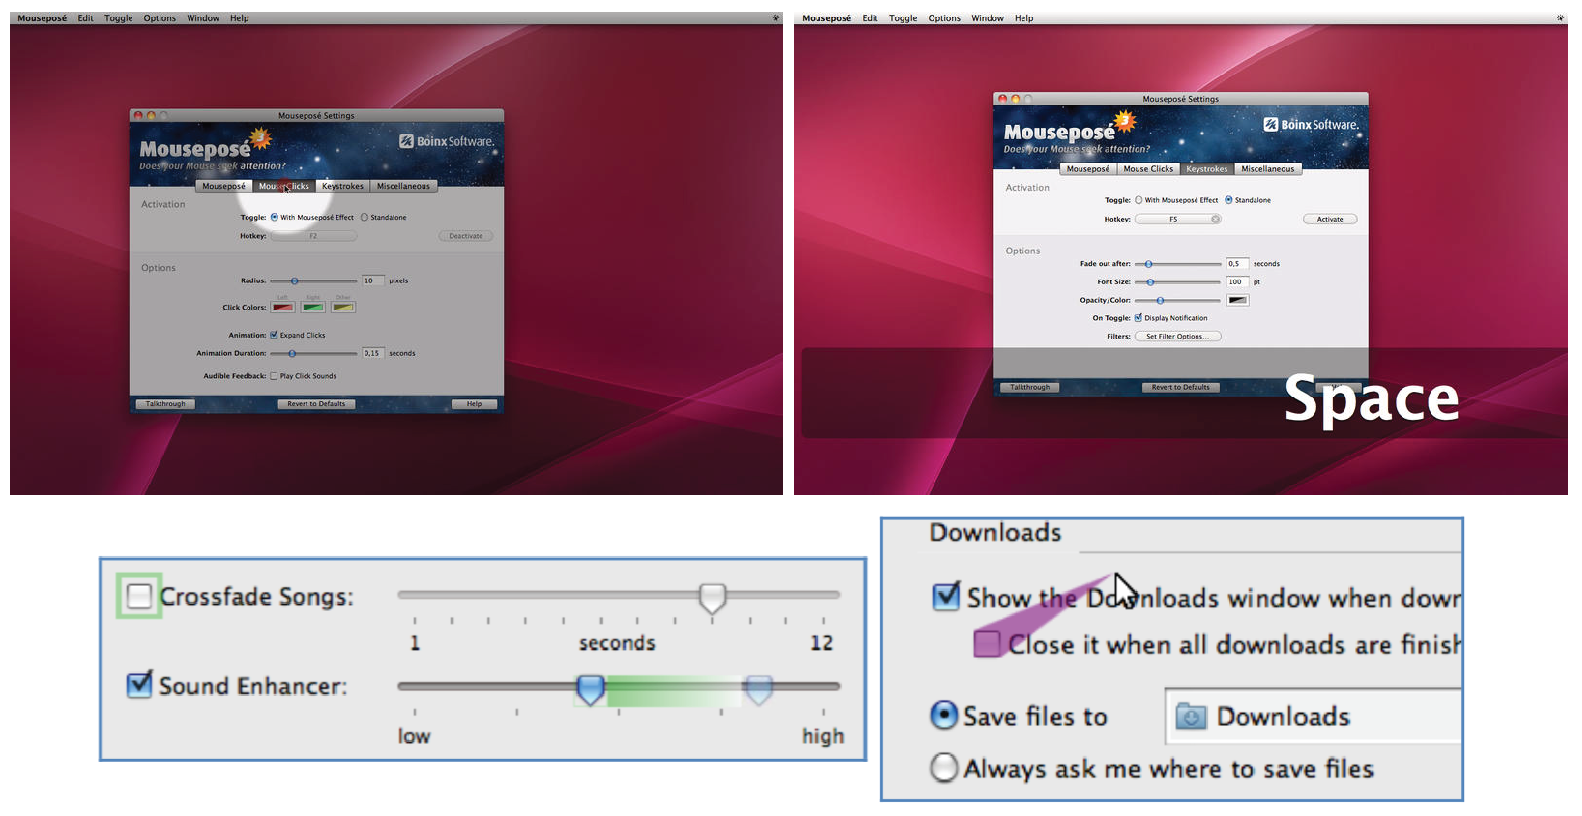
\includegraphics[width=0.7\textwidth]{\background/fig/realtime/realtime}
  \caption{Real-time visual enhancements on GUI applications: (top) Mouseposé highlights mouse cursors or text input; (bottom) Prefab creates target-aware or afterglow effects during user operating~\cite{Dixon:2010fb}.}
  \label{fig:related_realtime}
\end{figure*}

Real-time visual effects help users focus on the region of interest in a GUI application, but to support learners comprehend the application functionalities, there has been a considerable amount of research devoted to offering interactive helps.
%
Video snippets can be embedded in application tooltips~\cite{Grossman:2010wr}, which were shown to be seven times more effective than conventional tooltips for completing unfamiliar tasks.
%
Interactive, step-by-step instructions can be integrated in several forms:
%
To help user identify the correct UI components, tutorials can be shown via translucent colored ``stencils,'' which visually direct user's attention directly in an application~\cite{Kelleher:2005:STD:1054972.1055047}.
%
By tracking user's current operations, tutorials can be embedded in an application to provide instant feedback such as a check-mark or a percentage match~\cite{Fernquist:2011:SRE:2047196.2047245}, automatically replayed to provide the corresponding video instructions~\cite{Pongnumkul:2011ju}, or be shown as ambient help~\cite{Matejka:2011:AH:1978942.1979349}.
%
Instructions can be captured from demonstration as ``scripts'' for step-by-step navigation~\cite{Bergman:2005:DocWizards}. Having more user controls~\cite{Lieberman:2014:SML:2557500.2557543} or being enhanced with game elements~\cite{Li:2014:CGM:2556288.2556954, Dontcheva:2014:CCL:2556288.2557217} can further engage users in learning.

Last but not least, as tutorials are built for a broader community with a set of authors and learners, content can be dynamically updated within a community based on user contribution~\cite{Lafreniere:2013ff,Matejka:2009:CCR:1622176.1622214, Bunt:2014:TPI:2556288.2557118}.

interactive-visualization~\cite{Kwon:2016:CEO:2858036.2858101}
the paper that cited DemoWiz~\cite{Nguyen:2015:MST:2702123.2702209}

% These projects show how effective instructional representations can assist learners in learning or executing tasks. Our goal is to further study new formats that incorporate advantages of several formats of multimedia, including images, text, and videos, and in turn enhancing the learning experience for a variety of tasks.

% * define ``automatic''
% Note: MixT tutorials are automatically rendered from manual demonstration, not automatically generated.

% To provide real-time assistance, it is important to recognize the user activities during a task performance. Several domains have been widely studied, including software operations, scene recognition, and object tracking in a physical world.

% -------------------------------------------

\section{Instructions for Physical Activities}
\label{related_physical}

The above approach of tracking user behavior to automate tutorial authoring opens the door to interactive tutorials that can respond to user progress. However, tracking user behavior in the physical world, rather than in software, remains a challenge.

\subsection{Generating Instructions for Real-World Tasks}
Researchers have investigated tools for automatically generating visual instructions for physical tasks~\cite{feiner:1985:AEA:1299975.1300548,Seligmann:1991:AGI:127719.122732}. Workflows can be captured and created for furniture \cite{agrawala2003designing} or block assembly tasks \cite{Gupta:2012ku}.
%
If video content is difficult to be extracted, crowdsourcing algorithms have been introduced to structure step-by-step videos by online workers~\cite{Kim:2014:CSI:2611222.2556986}.
%
% New devices to support authors capturing multi-media materials, such as a turntable~\cite{Tseng:2015:SPT:2771839.2771869}
% documentation \cite{Tseng:2016:makeology}

\subsection{Interactive Guidance}
To provide responsive instructions, a computer system needs to understand user operations in real-time. Ideally, activities should be automatically tracked without human labeling.
%
Computer vision techniques can track specific physical targets, including hands \cite{Ranjan:2008}, user movements \cite{Wilson:2012fb}, fast-moving objects (e.g., a Ping-Pong ball) \cite{Okumura:2011tr}, or regions in pre-defined spaces \cite{Ranjan:2007}.
%
These methods usually require an expert defining heuristics of space regions or movement classifications ahead of time for the tracking program.
%
Thanks to the advance of technology, camera sensors such as Kinect have become widely available to track activities for block assembly~\cite{Gupta:2012ku} and dance~\cite{Anderson:2013:YEM:2501988.2502045}.

Real-time guidance is often shown via an external display, placed next to the working area~\cite{Gupta:2012ku}. To better blend the information into activities, Knibbe~\ea{} design a display-embedded table as a physical workspace that monitors, records, and assists users~\cite{Knibbe:2015:SMI:2817721.2817741}.
%
Alternatively, information can be overlaid on top of the work area using augmented reality, usually through a head-mounted display. Such systems can provide visual highlights for machine maintenance~\cite{Henderson:2011ff}, or interactive remote tutoring for repair tasks~\cite{Gurevich:2012ko}.
%
Another method is to overlay guidance on an augmented mirror for tasks such as dance movements~\cite{Anderson:2013:YEM:2501988.2502045}.

for Frisbee players~\cite{Solomon:2014:UTI:2540930.2540965}

% Lovell and Buechley use electrical sensing with conductive thread for a sewing tutorial~\cite{Lovell:2010tl}.

% I aim to propose a new approach that gives users flexibility in a home environment, and provides interactive control. If activity recognition is not possible, my approach includes users in the loop to annotate high-level information in order to create high-quality results.

% -------------------------------------------

\section{Working with Videos}

\tofix{intro here}

\subsection{Capture}
Several research and commercial systems guide users at capture time to yield higher-quality videos. Such systems often employ templates to help users capture sequences of distinct shots (e.g., Snapguide\footnote{\url{http://snapguide.com/}}) or suggest framing of the subject or camera view as in NudgeCam~\cite{Carter:2010}. Computer vision algorithms, like face tracking, can be used to offer real-time feedback during such directed actions~\cite{Davis:2003cu,Heer:2004ba,Carter:2010}. Instead of relying on templates, shot suggestions can also be bootstrapped through user dialogs~\cite{Adams:2005}.

\subsection{Annotation}
Researchers have investigated how to provide interactions that enable efficient, fluid annotation of video data, from the early EVA system~\cite{Mackay:1989} to more recent interfaces like VideoTater that leverage pen input~\cite{Diakopoulos:2006vt}.

\subsection{Editing}
Frame-based editing of video is very time-intensive, as it forces users to operate at a very low level of detail. Editors can leverage metadata, such as transcripts~\cite{Berthouzoz:2012,Pavel:2014:VDB:2642918.2647400} and shot boundaries~\cite{Casares:2002dx}, to give users higher-level editing operations at the shot level rather than the frame level.
In specific video domains like interview videos, transcripts can help users place cuts and transitions~\cite{Berthouzoz:2012}.
%
Computer vision techniques can automate certain effects, such as creating cinemagraphs~\cite{Bai:2012, Joshi:2012}, automatically-edited lecture videos~\cite{Heck:2007}, zoomable tapestries~\cite{Barnes:2010} and synopses~\cite{Pritch:2009vl}, or stabilizing shaky amateur videos~\cite{Liu:2011}. When analyzing video is a matter of subjective taste, identifying salient frames can also be outsourced to crowd workers~\cite{Bernstein:2011uj}.

live authoring through compositing and editing of streaming video~\cite{Freeman:2014:LLA:2611105.2557304}

\subsection{Navigating}
Videos can be navigated at the content level beyond log events, such as visualizing subject movements in a storyboard design \cite{goldman2006schematic} and enabling direct manipulation of a target in 2D \cite{Dragicevic:2008:VBD:1357054.1357096,Goldman:2008:VOA:1449715.1449719,Karrer:2008:DDM:1357054.1357097} or 3D \cite{Nguyen:2013:DMV:2470654.2466150}. These techniques help viewers understand content flow and playback videos, and have been applied to screencast videos \cite{Denoue:2013:RDM:2451176.2451190}. It is also possible to automate video control based on user actions for scenarios such as operating software applications~\cite{Pongnumkul:2011ju} and block assembling tasks \cite{Gupta:2012ku}. Such novel forms of video navigation inspired us to explore new visual designs for revealing the video content that support live presentations.

lecture videos~\cite{Tang:2006:DIU:1111449.1111523}

Visualization of personal history for video navigation~\cite{Al-Hajri:2014:VPH:2611105.2557106}

% In contrast to these systems, we do not require the author to manipulate the camera or system during capture. Many leisure activities, such as home repair or cooking, require use of both hands or involve getting one's hands dirty, so camera manipulation is not possible. We use vision techniques for automatic recording and editing. It differs from previous approaches in its focus on particular application domains -- software and physical demonstrations. By focusing on specific domains, we can make assumptions about the structure of the input and output video, such as the fact that there is a linear set of steps or movements, and offer user interfaces and algorithms that make it easier to create high quality instructions.

%!TEX root = ../thesis.tex
\section{Design Guidelines}

Researchers provide different findings on the effectiveness of media formats of software tutorials. Evaluating the instructional potential of videos began in the 1990s. Palmiter, Elkerton [16,17], and Harrison [11] studied the effect of animated demonstrations on learning and instruction recall. More recently, Grabler et al. compared how users followed book tutorials, videos, and automatically generated static tutorials [8]. Their results showed that automatically generated text and image tutorials outperformed video or book instructions on time and errors. Grossman et al. studied the effectiveness of embedding short (10-25 second) video clips in applications [9]. They found that participants who had access to video-based tooltips were significantly faster in completing tasks than those who viewed static ones.

While these studies suggest that there is still some debate over the tradeoffs between step-by-step static and video tutorials, they provide strong support for two key claims: step-by-step tutorials help users make fewer errors by allowing them to work at their own pace, while videos can help provide subtle details of complex interactions that are difficult to represent statically. Based on these findings, we designed a formative user study that investigates whether video clips can be incorporated into a step-by-step framework to help users follow certain types of image-editing tasks within a tutorial.

\subsection{Formative User Study}

\begin{figure*}[t]
  \centering
  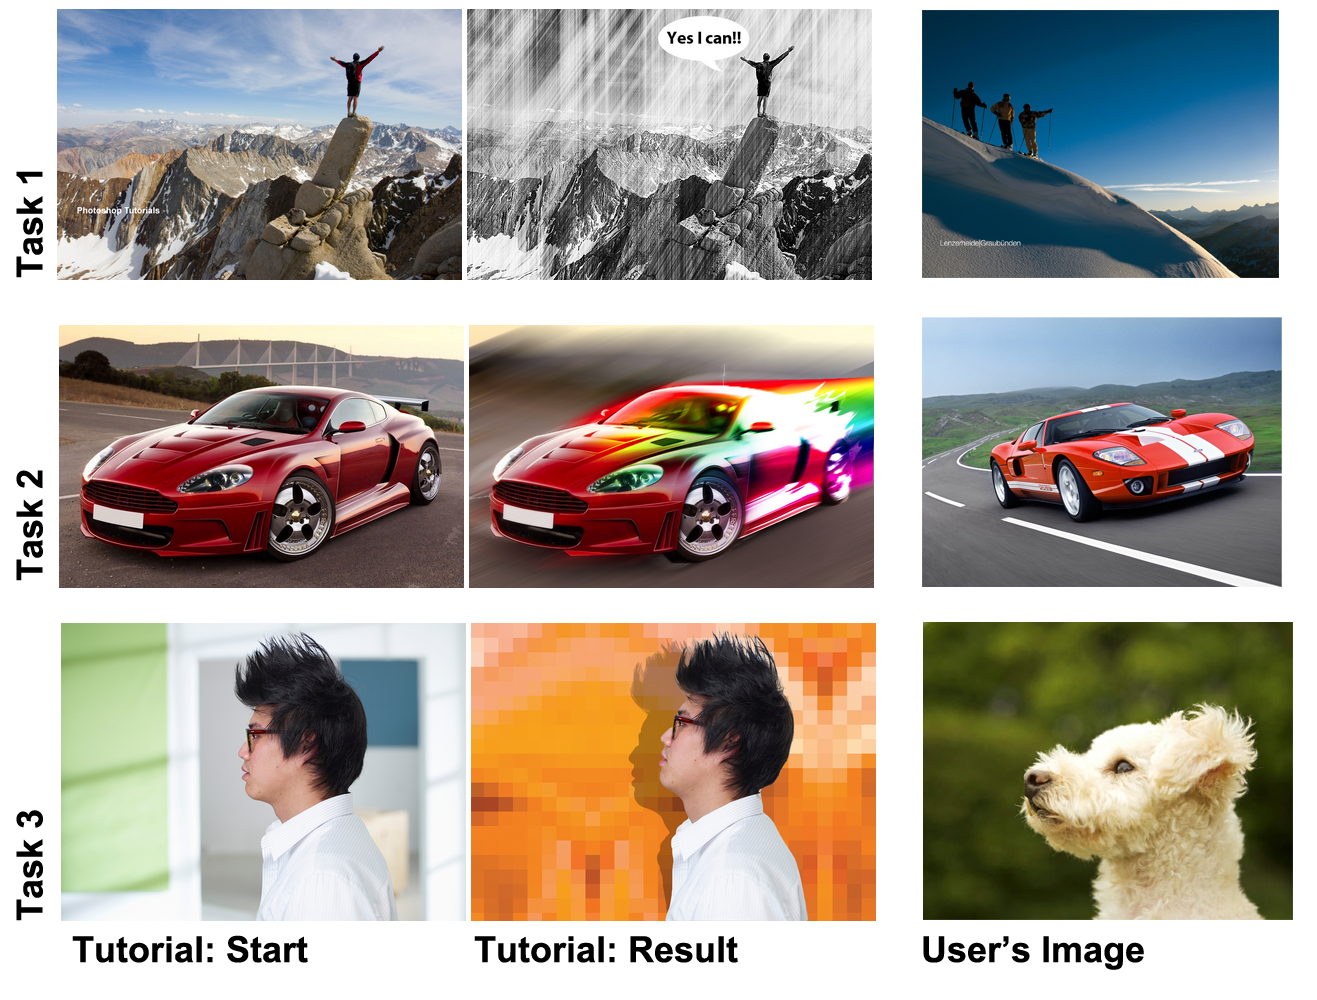
\includegraphics[width=\textwidth]{\mixt/fig/formative_study/study-images}
  \caption{In our formative study, participants completed three tutorials with images similar but not identical to the originals.}
  \label{fig:formative_tasks}
\end{figure*}

\begin{figure*}[t]
  \centering
  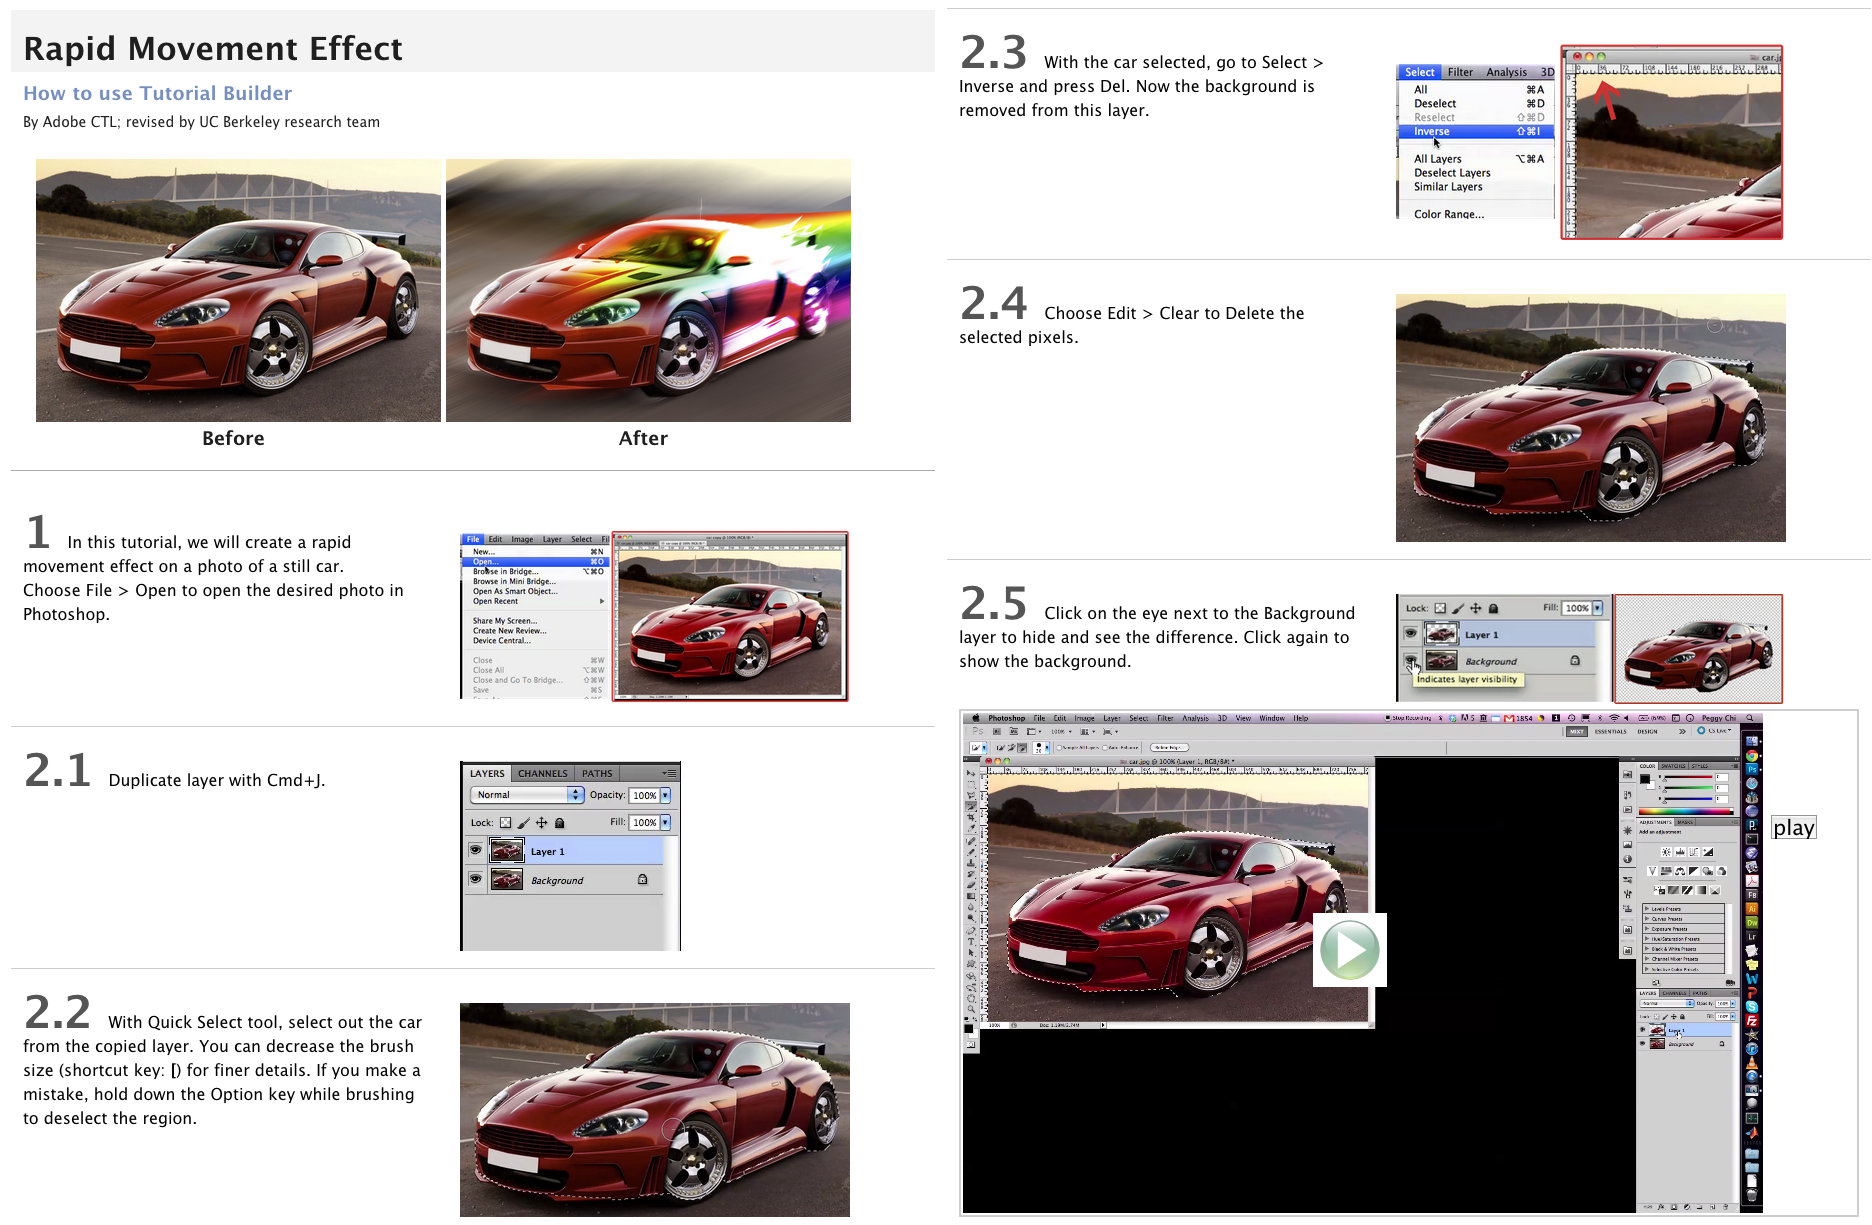
\includegraphics[width=\textwidth]{\mixt/fig/formative_study/study-mixed-example}
  \caption{In the mixed condition, participants saw an HTML page with static images and text; they could expand each step to view a video of that step (here: step 2.5).}
  \label{fig:formative_mixt}
\end{figure*}

% \subsubsection{Study Design}
\subsubsection{Hypothesis}
Our formative study aims to test the following two hypotheses:

H1: Image manipulation tutorials that mix static images and video clips are more effective than all-static or all-video tutorials.

H2: Users benefit more from seeing video clips instead of static text and images for certain types of commands.

\subsubsection{Participants}
We recruited 12 participants (5 males and 7 females, aged 20-52), 4 from a campus student design group and 8 from a computer software company, and compensated each with a \$15 gift card for participating. Our tutorials focused on achieving specific tasks in Adobe Photoshop. We recruited participants who had prior expertise with Adobe Photoshop, but who were not expert users. To demonstrate expertise, potential participants first completed an online screening test that asked them to follow a short image manipulation tutorial and submit the resulting file. The selected participants had between 1 and 20 years of experience using Photoshop.

\subsubsection{Tasks and Material}
The study was based on a within-subject design. We looked through Photoshop books and selected 3 different image manipulation tasks with similar levels of difficulty and complexity (see Figure~\ref{fig:formative_tasks}). Each tutorial comprised 15-20 steps. We focused on tutorials that included new, less common features such as the liquify tool, gradient warp tool, and puppet warp tool to increase the chance that participants would encounter unfamiliar tools. For each tutorial, we created three types of presentations: 1) static (in HTML format displayed on the screen), 2) video (on YouTube with audio narration), and 3) mixed (web interface shown in Figure~\ref{fig:formative_mixt} without audio). To ensure that different formats presented equivalent information where possible, we first recorded and narrated our video tutorials, then manually generated the static version by writing text instructions based on the narration and annotating and cropping frames of the video. To create mixed tutorials we started with the static tutorials and added the corresponding screencapture video segment for each step. To view the video segment for a step in the mixed tutorial, the user had to click on the image for that step. We scaled these videos to a fixed resolution of 800x500 pixels so that at least 2-3 steps would fit on screen when the videos were expanded. Many online tutorials do not offer full-screen resolution videos; even when high-resolution videos are available, they are hard to use as they force users to continually switch between the video and application windows. We disabled the soundtrack in the mixed tutorial to avoid situations when users only relied on auditory instructions instead of learning from static or video formats.

For each task, participants were given a source image that was distinct, but thematically similar to the image manipulated in the tutorial itself. This study design choice was motivated by the fact that users typically want to transfer the techniques found in tutorials to their own images.

\subsubsection{Procedure and Environment}
Each session consisted of 1 warm-up task and 3 experimental tasks. The warm-up task was a short 5-step static tutorial. In the 3 experimental tasks the format and task order were randomized. Each 60-minute session was conducted in a lab environment, using computers running Mac OS X, Adobe Photoshop CS5.1 and a web browser (Google Chrome) for viewing tutorials. Each participant was provided with a keyboard and a mouse and was allowed to adjust the equipment setting such as the monitor position and mouse tracking speed during the warm-up task. Photoshop and the web browser were arranged side-by-side on a 30-inch monitor with a resolution of 2048x1280 pixels. During the study, we used screen capture software to record user performance.

\subsubsection{Measurement}
To evaluate H1, we report the number of errors and repeated attempts that the participants made for each task. While our ultimate goal is skill acquisition and retention, we focus on the pragmatic goal of improving users' success in following tutorials and performing the instructions. We record an error if the participant performed a command incorrectly or skipped a step in the tutorial. While errors give a sense for the effectiveness of the tutorials, they do not measure the extraneous work users might have to perform when they have trouble understanding the correct outcome of a step. For example, if a user makes an error and then correctly executes several steps before recognizing the problem, we count this as a single error, even though the user must go back to fix the problem and then redo the subsequent steps. In addition, users may select the right command, but be dissatisfied with the result of their image and try again (e.g., redrawing a gradient). In such cases, we record all executions of the same step following the first attempt as a repeated attempt. Note that we do not count adjustments of continuous parameters or refinements of selection regions as repeated attempts because in these cases, the user is focusing on a single action rather than repeating a previously executed step. We do count a repeated attempt if the user entirely undoes a step to then retry it.

To evaluate H2, we count the number of different users who click on the video for each step in the mixed tutorials. To determine whether some types of commands benefit from videos more than others, we bin each step into one of the following five command categories based on the types of user interaction and UI elements it involves: brushing/drawing, manipulating control points (e.g., mesh-based warping, spline editing), parameter adjustment (e.g. using a slider to change opacity), UI navigation (e.g., switching tools, finding menu items), and layer operations.

We also collect qualitative data by observing how users follow the presented information and obtain additional feedback via 5-point Likert-scale questions (e.g., “The {\textless}condition{\textgreater} tutorial was easy to follow.”) and open-ended questions (e.g., “Compared with static tutorials, what were the pros and cons of the mixed media tutorial?”).

%!TEX root = ../thesis.tex

\subsection{Design Implications}

Based on our analysis of existing video tutorials and interviews with
tutorial authors, we identified a few key aspects of the tutorial creation
process that have important design implications for DIY video
editing systems.

\subsubsection{Working with single take, single camera footage.}
%
Most amateur authors record demonstrations in a single take with a
a single camera. As a result, the captured footage often includes
mistakes and long, repetitive actions.

\subsubsection{Making concise videos.}
%
The most important design principle for creating effective DIY videos
is to make them concise without sacrificing clarity. To this end,
authors remove/condense unnecessary or repetitive actions so that the
resulting video only contains salient footage.

\subsubsection{Retiming audio and video tracks separately.}
%
One common technique for speeding up a video involves breaking the
synchronization between the audio and video tracks so that they can be retimed
separately. In cases where the narration refers to
specific visual events, the tracks should remain aligned.

\subsubsection{Emphasizing important information.}
%
Most effective DIY videos include titles, annotations and/or closeup
views to emphasize relevant information and highlight key details.

\subsubsection{Focusing on high-level editing decisions.}
% Editing captured footage is a difficult and time-consuming task.
Amateur users often struggle with low-level manipulation of cut points and timing in general-purpose video editors: A system should reduce the editing efforts and enable authors to focus on making simple choices for the final production.

We next describe how these considerations informed the design of DemoCut.

%!TEX root = ../thesis.tex
\section{Authoring}

\begin{figure}[b!]
  \centering
  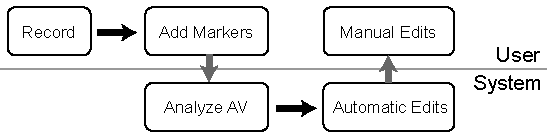
\includegraphics[width=0.7\columnwidth]{\democut/fig/block-diagram}
  \caption{DemoCut users first mark their recorded video in the Annotation Interface. DemoCut then segments their recording and suggests video edits, which users can review and change in the Editing Interface.}
  \label{fig:block-diagram}
\end{figure}

To enable amateur users to produce effective video tutorials, the DemoCut video authoring system semi-automatically edits a long, single take recording into meaningful steps.
Early testing revealed that users find it easier to locate specific {\em moments} in the video than to mark or edit {\em segments}. Therefore, our Annotation Interface asks users to mark important moments.
%
DemoCut combines the user annotations with audio and video analysis to automatically generate a segmented video with editing suggestions:
%
It removes or condenses unnecessary/repetitive actions and enables flexible synchronization between audio and video tracks.
Titles, visual annotations and closeup views are applied to enhance the content.
%
Users can review and revise these decisions in the DemoCut Editing Interface.
This section reviews DemoCut from the user's perspective (Figure~\ref{fig:block-diagram}). The following section will describe our video analysis pipeline.

\begin{figure*}[t!]
  \centering
  \includegraphics[width=0.7\columnwidth]{\democut/fig/ui_annotation}
  \caption{With DemoCut's Annotation UI, users add markers to their recorded video (A). Each marker can be labeled with a descriptive string (B).}
  \label{fig:ui_annotation}
\end{figure*}

\subsection{Annotating the Video}
The purpose of the DemoCut Annotation UI is to collect high-level information that is difficult to extract automatically but useful in determining how to edit the video.
We rely on users to distinguish important from unimportant actions and successful steps from mistakes.
The user scrubs through the captured footage and adds markers for distinct moments, such as the instant when he cuts a sheet of paper (Figure~\ref{fig:ui_annotation}A). DemoCut offers five types of markers for annotating a video:
\begin{itemize}
  \item \emph{Step}: indicates the start of a major part of the task
  \item \emph{Action}: marks important moments
  \item \emph{Closeup}: indicates moments where the action is happening in a small region of the video frame, e.g., for a detailed action such as fastening a small screw. %User can specify a zoom region.
  \item \emph{Supply}: indicates a tool or material used in the task
  \item \emph{Cut-out}: indicates moments of the video that should be removed due to occlusion or a mistake in the performance.
\end{itemize}
This set of markers was derived from our observations of the structure of effective tutorial videos: actions are treated separately from supplies; zooming can direct the viewer's attention to a small area of the frame; and step divisions are used to divide actions into meaningful groups. Rather than specify start and end frames, users can place a marker on any frame of an important moment.
%Each genre of video will likely have a different set of semantic markers.

Users can add descriptions to markers (Figure~\ref{fig:ui_annotation}B). These descriptions serve a dual purpose: they are used to generate automatic subtitles, and they are also shown as segment names in the Editing Interface to facilitate navigation. Users can also add visual highlights such as boxes and arrows to any marker.
%The collected meta-data is then used for later analysis.

\subsection{Automatic Video Editing}
Based on the user's markers, DemoCut automatically segments the raw footage and applies editing effects using the following techniques.
%To automatically segment the video, DemoCut uses two types of analysis. First, it looks for changes in the video around markers using frame differencing. Second, it detects narration through audio analysis. It combines the video and audio analysis to select appropriate editing effects from two classes: temporal effects and visual effects. The user can change effects selected by the system in the Editing Interface.

\begin{figure}[b]
  \centering
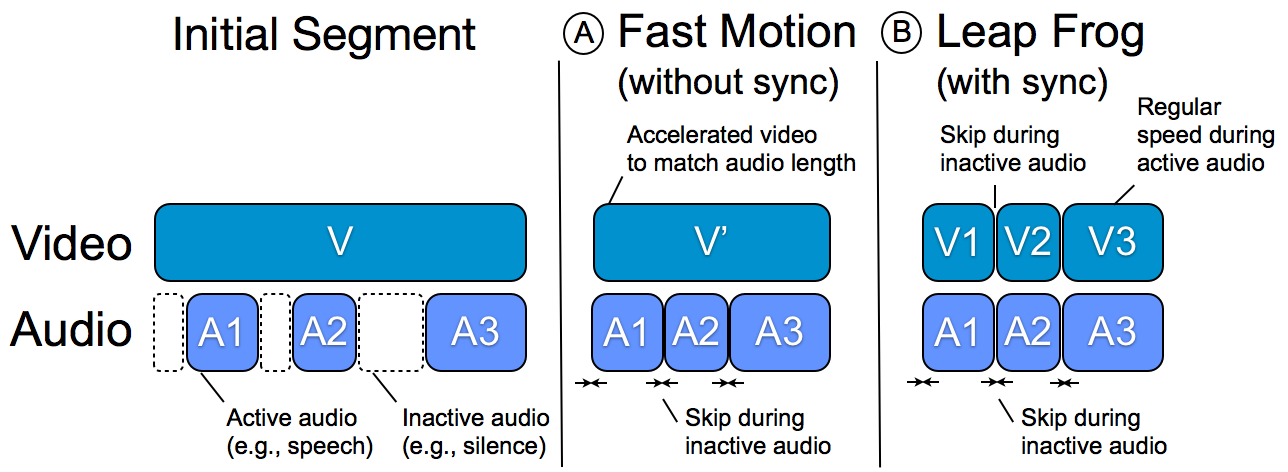
\includegraphics[width=0.7\columnwidth]{\democut/fig/fastmotion}
  \caption{DemoCut accelerates playback of video with intermittent audio narration through Fast Motion (A) and Leap Frogging (B).}
  \label{fig:fastmotion}
\end{figure}

\subsubsection{Temporal Effects}
We designed four temporal effects to shorten a video. In addition to skipping a segment or leaving it unchanged, we consider the synchronization between the audio and video tracks: People are sensitive to changes in speech playback speed, but video can often be accelerated without loss of clarity. Therefore,
%-- especially of idle time, slow or repetitive movement --
%\bh{We know this intuitively, would be nice to find a reference}.
our temporal effects accelerate or contract video but keep audio at normal speed.

{\em Fast motion (with merged audio)}: When a segment includes several sections of narration with intermediate pauses, DemoCut removes the pauses and concatenates the audio segments. Then it speeds up the video so the total video length corresponds to the length of the concatenated audio (Figure \ref{fig:fastmotion}A). This effect is appropriate if tight synchronization between audio and video is not required. For example, an author may describe general strategies for choosing supplies while measuring paper -- here audio and video are independent of each other. In this case, DemoCut will accelerate the video %of salad mixing
to fit the length of the author's remarks.
%This is our default effect.

{\em Leap frog (with synchronized audio)}: If synchronization between audio and video is necessary, this effect plays video and audio at normal speed during active audio segments, and skips video in the interstitial segments (Figure \ref{fig:fastmotion}B).
Synchronization is important if the author's face is in the shot (so lip movement and audio match), if actions produce distinct sounds (like cutting paper), or if the narration refers specifically to actions, e.g., when pointing at an object and describing its properties.
Since DemoCut cannot automatically decide whether synchronization is necessary,
% and it tries to aggressively shorten the video,
it applies the Fast Motion effect by default but offers users control to change that effect.

{\em Skip:} Depending on the length of the removed segment, DemoCut either applies a fade through black (for segments up to 15 seconds); or a fade to a title that indicates how much time has passed (e.g., ``2 minutes later'').

If these temporal effects are not appropriate, DemoCut plays the audio and video at the captured rate. We call this the {\em Normal} effect.

\begin{figure*}[t!]
  \centering
  \includegraphics[width=0.85\columnwidth]{\democut/fig/ui_editing}
  \caption{DemoCut's Editing Interface shows automatically generated segments with effect suggestions (A). Users can change the effect (B) applied to each segment (C).}
  \label{fig:ui_editing}
\end{figure*}

\subsubsection{Visual Effects}
In addition to manipulating time, DemoCut offers three visual effects to structure the video and to provide emphasis. These visuals appear for the duration of the segment DemoCut derived from the user's marker:

{\em Subtitles}: Text entered by the user in the marking phase is converted into automatic subtitles with two levels -- a step heading that remains on screen for all segments within a step (e.g., ``Wrapping the present''); and a subheading from individual event markers (e.g., ``Sharpen creases'').

{\em Automatic zoom}: When users create closeup markers, they also specify a rectangular region of interest. DemoCut automatically crops and enlarges this region of the segment.

{\em Visual annotation}: DemoCut overlays visual box or arrow annotation specified by the user in the marking stage.

\subsection{Reviewing and Editing}
Since our automatic video and audio segmentation has a limited understanding of the video, it is likely that some editing decisions will be incorrect. For example, DemoCut's algorithms have no way of inferring whether audio-video synchronization will or will not be required in a given segment. In addition, automatic analysis may also lead to errors: if the narration is not correctly segmented, speech can be cut off mid-sentence. DemoCut's editor gives authors the opportunity to review and revise all editing decisions.

In the Editing Interface, the video is visualized as a set of segments (Figure \ref{fig:ui_editing}C) flowing from top to bottom on the right side of the main video view (Figure \ref{fig:ui_editing}A). There is no traditional timeline for two reasons: first, editing operations only apply to detected segments (we consciously prevent users from applying frame-level edits to keep with the goal of a semantic editor); second, because segments may come with labels entered by the user, a vertical layout makes it easier to read labels. Users can navigate to any segment by clicking on its thumbnail. Once selected, they can change which effect should be applied to a given segment (Figure \ref{fig:ui_editing}B). Users can also modify any visual effects, to edit subtitles, resize the cropped region, or add/delete highlights. When satisfied with their choices, users can export a continuous video suitable for online video sharing platforms.

%\subsection{Tutorial Outputs Formats}
%\bh{Cut, shorten or merge with previous?}
%Finally, DemoCut produces the edited video in three formats:
%\begin{itemize}
%  \setlength{\itemsep}{0pt}
%  \item \emph{Video only}: a complete video clip with subtitles and effects for video %sharing platforms.
%  \item \emph{Indexed video}: a video player with markers below the timeline, similar to %the DemoCut Annotation UI. Viewers can navigate to a specific instruction via the marker %buttons.
%  \item \emph{Step-by-step instructions}: a series of mixed-media instructions on a web %page. Researchers identified how ... \cite{Chi:2012:MAG:2380116.2380130}.
%\end{itemize}

% \bh{say something about exporting in different formats?} \pc{move this subsection back from future work}

%Answer: why not provide visual sense of time

%visualize timeline: modified from timeline.js \cite{Cazenave:2011dg}
%\bh{I don't think you want to describe this as a UI for the author - this is a debugging tool for us and a %tool to explain the analysis through figure in the next section}.

%!TEX root = ../thesis.tex
\section{Automatic Effect Decision Pipeline}
DemoCut performs several automated steps to convert the user-annotated
input recording into an edited video tutorial. First, the system segments the recording into regions around user-specified markers. This segmentation considers both the
similarity of video frames around each marker and the presence of
narration in the audio track in order to determine the appropriate
segment boundaries (Figure~\ref{fig:democut_pipeline}). DemoCut then automatically applies an temporal and a visual effect to
each segment based on the type of the corresponding user marker and
the properties of the audio/video content in the segment. The rest of
this section describes these steps in detail.

\begin{figure}[t]
  \centering
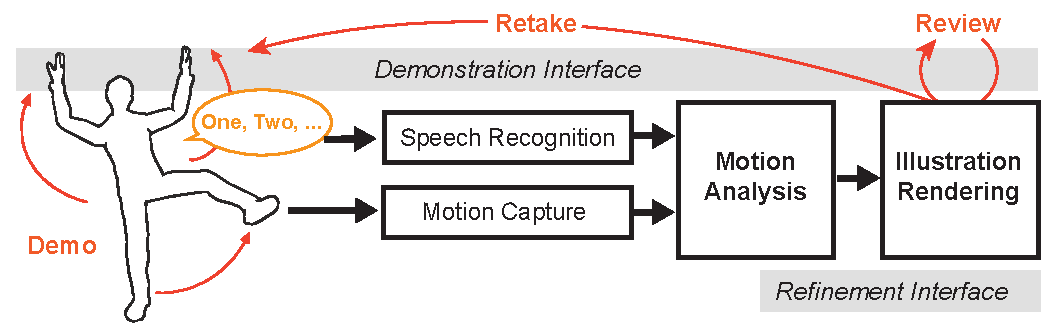
\includegraphics[width=0.8\columnwidth]{\democut/fig/pipeline}
  \caption{Given user markers, DemoCut analyzes both video and audio to segment the demonstration video and apply editing effects.}
  \label{fig:democut_pipeline}
\end{figure}

\subsection{Video Segmentation}

Except for the step marker, all of the user-specified markers indicate
important moments in the demonstration that correspond to some segment
of the recording. In many cases, we can infer the duration of these
segments by searching for video frames that look similar to the marked
frame. For example, in Figure~\ref{fig:video-similarity}A, the similar
frames before and after a supply marker show the author holding up a
bottle of vinegar, and in Figure~\ref{fig:video-similarity}B, the
similar frames around an action marker show the author grating cheese.
%
For every marked frame $T^m$, DemoCut uses the following method to
compute candidate start and end frames $T^s$ and $T^e$ for the
corresponding segment.
%
For the $i$-th marked frame $T_i^m$, our algorithm finds $T_i^s$ by
comparing $T_i^m$ to earlier frames in the video until it reaches a
previous marker at $T_{i-1}^m$, or until 5\% of pixels (in grayscale)
%in the grayscale versions of the frames
have changed by 20\%. Similarly, the system
finds $T_i^e$ by comparing $T_i^m$ to subsequent frames in the video.
To optimize performance, DemoCut compares to frames sampled at 0.5
seconds and ignores overlaps between segments. Segment overlaps are
resolved during boundary adjustment after incorporating the audio
analysis.

\subsection{Adjusting Segments with Audio Analysis}

Adjacent segments can have different effects that change how video and audio are processed. To prevent such changes from interfering with a video's narration, DemoCut adjusts segment boundaries to align with audio activity boundaries.
% DemoCut chooses different editing effects for different
% segments. Segment boundaries should therefore be carefully adjusted based on the audio
% track to avoid interrupting the author's narration.

\subsubsection{Detecting non-silent sections}
%
Since many DIY videos include prominent non-speech sounds such as
chopping noises, power tools, etc., detecting speech automatically is
a challenging task. We found that even state-of-the-art speech
detection algorithms produce poor results in many cases.
%
As a result, we take a more conservative approach; DemoCut
automatically detects non-silent sections in the recorded
audio and treats the background sound as part of the narration.

At a high level, our algorithm for detecting non-silent sections works
as follows. We compute the ``loudness'' of each audio window,
organize the windows into a histogram based on loudness, and then
analyze the histogram to determine a minimum loudness threshold for
non-silent windows. We then apply this threshold to categorize all
audio windows as silent or non-silent. Finally, we filter this
categorization to eliminate very short sequences of silent or non-silent samples. Here, we describe these steps in more detail:
% \bh{I think we mean "window" instead of "sample" for the preceding section, since RMS operates on windows.}

\emph{Computing loudness.} Given an input audio waveform sampled at
44.1 kHz (Figure~\ref{fig:audio}A), we estimate loudness by computing
the root mean square (RMS) energy~\cite{Panagiotakis:2005eb} across
the entire waveform. The RMS energy
for a window of size $n$ is $\sqrt{(\sum_{n}{x_i^2})/n}$ where $x_i$ is the value of
the $i$th audio sample in the window. We set window sizes as 0.1 second with $n = 4410$. Prior to computing RMS energy, the audio is normalized and noise-reduced with Adobe Audition.

\begin{figure}[t]
  \centering
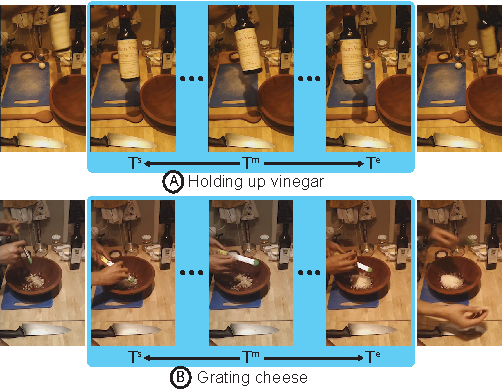
\includegraphics[width=0.6\columnwidth]{\democut/fig/video-similarity}
  \caption{DemoCut looks for similar video frames before and
after a marked frame $T^m$ to find candidate start ($T^s$) and end ($T^e$) frames
for the corresponding segment.}
 \label{fig:video-similarity}
   \vspace{-0.05in} %bjoern: at -0.25, fig 8 below cuts off caption text of this fig
\end{figure}



\emph{Computing loudness threshold.} After analyzing the RMS energy
profiles of several different types of DIY videos, we found that the
vast majority of recorded audio represents background sound, which
tends to have similar and fairly low RMS energy values. In contrast,
user narration varies from medium to high RMS values based on the
speaker's distance to the microphone and the sensitivity of the
recording device. Based on this observation, we first compute a histogram
of RMS energy for all windows in the audio track; the windows that
correspond to background sound form a large mass at the low-RMS end of
the histogram (Figure~\ref{fig:audio}B).
%
To distinguish these ``silent'' parts of the recording from the
narration, we smooth the histogram with a Gaussian kernel, find the
minimum derivative point in the smoothed histogram, and set the
loudness threshold $\varepsilon$ to be the RMS energy value at this
elbow point.
%
Figure~\ref{fig:audio}B shows the RMS histogram and loudness threshold
for one of our example videos, ``How to make salad dressing.''

\emph{Categorizing silent/non-silent sections.} To partition the audio
track into silent and non-silent sections, we first label each window
as silent or non-silent based on $\varepsilon$.
%
This initial labeling often includes some very short silent and
non-silent sections.
%
Since many short silent sections correspond to short pauses between
spoken words, we turn any silent sections that are shorter than 0.4
seconds into non-silent sections.
%
Then, we discard any non-silent sections that are shorter than 0.8
seconds to account for any clicks and pops in the recorded audio.
%
The 0.4 and 0.8 second thresholds for silent and non-silent sections
were tuned experimentally, and we used these parameter values for all
of our results.
%
%To filter out short silent pauses between spoken words, we smooth the labeled array using a sliding window of 0.5 second: if there exists a silent label $L_0$ between two non-silent labels $L_1$ in a sliding window, flip $L_0$ to $L_1$. Finally, we segment the smoothed labeled array by finding consecutive non-silent labels $L_1$ and save as a list of non-silent sections {[$S_1^s$, $S_1^e$], [$S_2^s$, $S_2^e$], \ldots, [$S_m^s$, $S_m^e$]} (Figure \ref{fig:audio}C).

\begin{figure}[t]
  \centering
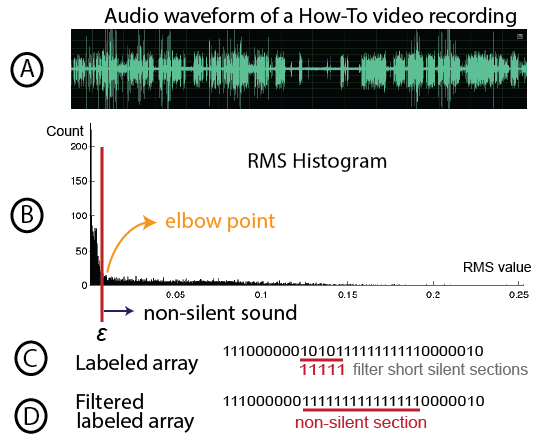
\includegraphics[width=0.8\columnwidth]{\democut/fig/audio}
  \caption{We use RMS energy of the audio to find silent and non-silent regions. We determine the threshold for silence by analyzing the histogram of the RMS energy.}
  \label{fig:audio}
\end{figure}

\subsubsection{Adjusting segment boundaries}

In order to avoid cutting off an author's narration, DemoCut
adjusts the video segment boundaries using the non-silent sections
of the audio track (Figure~\ref{fig:democut_pipeline}). First, for any segment
%[$T_i^s$, $T_i^e$]
we find
all of the overlapping non-silent audio sections and then grow the
segment so that it completely contains all of these non-silent sections.
%
Next, DemoCut resolves overlapping segments: If any two segments
overlap,
%such that $T_{i}^{e} > T_{i+1}^{s}$,
the boundaries must be readjusted.
%
If the overlap region is silent, the region is split into two equal parts and each is assigned to the
corresponding segment.
%
If the overlap region includes a non-silent audio section,
DemoCut assigns this non-silent section to the segment that has
more overlap with the section. If the overlap for both video segments is the same, DemoCut assigns the section to the smaller video segment.
%
Finally, DemoCut addresses any gaps between segments. If a gap is less
than 2 seconds, it is merged to the shorter adjacent segment.
Otherwise, DemoCut creates a new segment for the gap. Note
that such {\em unmarked segments} do not have a corresponding marker, but
they may still show useful details of the demonstration.


%Using the non-silent sections of the audio track, DemoCut adjusts the video segment boundaries for each user-specified marker (Figure \ref{fig:audio}C). For a marker at $T_i^m$ with a shot boundary [$T_i^s$, $T_i^e$] where  $T_{i}^{s} > T_{i-1}^{e}$ and $ T_{i}^{e} < T_{i+1}^{s}$, we find all the overlapped non-silent sections during this time interval: {[$S_j^s$, $S_j^e$], [$S_{j+1}^s$, $S_{j+1}^e$], \ldots, [$S_{j+k}^s$, $S_{j+k}^e$]}.
%
%In order to have each video segment contains complete narration without a sound cutoff, we examine the first and last non-silent section and adjust the segment boundary to [$ min(T_{i}^{s}, S_{j}^{s}), max(T_{i}^{e}, S_{j+k}^{e}) $].
% Note: avoid sound cutoff if a segment is "skipped"

%After all the annotated segments are adjusted, for any two consecutive segments where their boundaries are overlapped that $T_{i}^{e} > T_{i+1}^{s}$ by $x$ seconds, if they share one speech section [$S_j^s$, $S_j^e$], assign this speech section to the video segment that overlaps more and adjust the start and end frames, i.e. either $T_{i}^{e'} = S_{j}^{e}$ or $T_{i+1}^{s'} = S_{j}^{s}$ so that $T_{i}^{e'} < T_{i+1}^{s'}$. If there is no speech section in the overlapped time frame, split into half, i.e. $T_{i}^{e'} = T_{i}^{e} + x/2$ and $T_{i+1}^{s'} = T_{i+1}^{s} - x/2$ (Figure \ref{fig:audio}D).

%In order to completely segment the entire recording, for any gap between annotated segments, if it falls below 2 seconds, merge to the shorter adjacent segment; otherwise, create an empty segment (Figure \ref{fig:audio}E).

\subsection{Applying Effects}

To automatically apply an effect to each
computed segment, DemoCut first detects whether
there is motion in the video. A segment is considered to be {\em static}
(i.e., no motion) if less than 1\% of pixels in the grayscale versions
of consecutive frames have changed by more than 20\%. To optimize for
performance, the segment is sampled at 0.5 seconds for this
comparison.
%
DemoCut chooses effects as follows:

\begin{enumerate}
  \item If the segment includes a \emph{cutout} marker, apply {\em ``Skip''}.
  \item If the segment includes a \emph{closeup} marker, apply {\em ``Zoom''} to the entire segment.
  \item If the segment includes any non-silent audio sections, apply {\em ``Fast Motion''}.
  \item If the segment is silent, static, and unmarked, apply {\em ``Skip''}.
  \item If the segment is silent but not static (either marked or unmarked), apply {\em ``Normal''}.
  \item For any marker with a text annotation, apply {\em ``Subtitles''}.

  \end{enumerate}
% \bh{Missing discussion of how to apply zoom and subtitles here. I think zoom is applied to the whole shot, while there are two levels of subtitles - one for the step level, and one for a shot/segment level.}

%These rules result in a default set of editing effects for the entire
%video tutorial. The information is saved as metadata to playback in the Editing UI. As described in the previous section, users can manually change the editing effect for any segment.

%!TEX root = ../thesis.tex
\subsection{Implementation}
Kinectograph is implemented in C\# using the official Kinect API and the Arduino software. Our Tablet UI is implemented with the standard Web technologies, including HTML5, CSS3, JavaScript, and jQuery for recognizing touch gestures and communication.

% The tablet UI was built using HTML5/JavaScript. This communicated to t
% C\# program, Kinect API, Node.js server, HTML5/JavaScript web UI on iPad \pc{To write}

%!TEX root = ../thesis.tex
\section{Evaluation}

\begin{figure}[t]
  \centering
  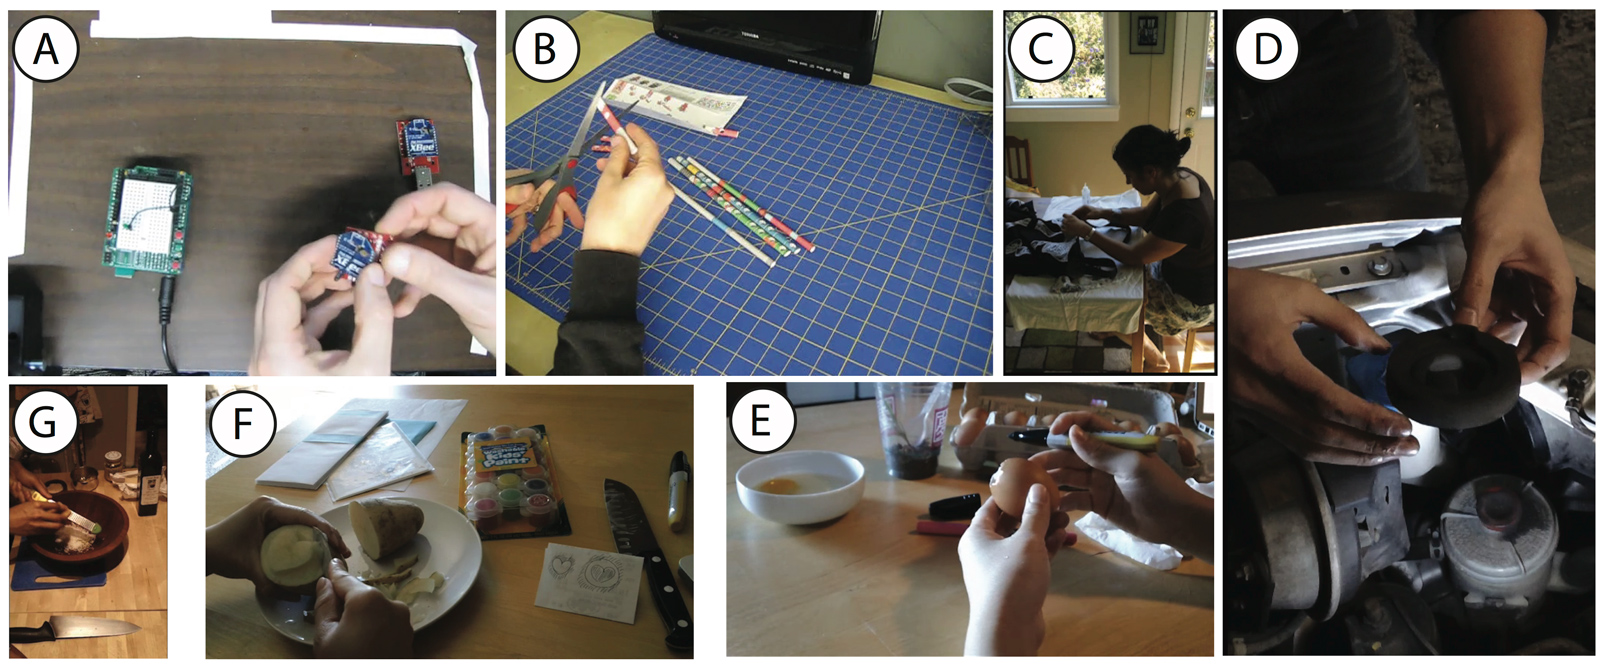
\includegraphics[width=\columnwidth]{\democut/fig/results-small}
  \caption{Illustrative frames from the seven videos used to assess DemoCut. Labels correspond to task labels in Table~\ref{tab:system_results}.}
  \label{fig:results}
  \vspace{-0.2in}
\end{figure}

\subsection{Evaluating Automatic Effect Decision}

To evaluate DemoCut's analysis engine, we recorded seven how-to tasks
from the five categories we selected in the formative user study
(Table~\ref{tab:system_results}).
%
The tasks were recorded by 4 people (all authors of this
work) in 7 locations using a Sony camcorder or an iPad with
a video resolution of at least 640x480 pixels.
%
We used DemoCut to annotate the recordings and then examined the
automatically generated tutorials.

Overall, the resulting tutorials exhibit many of the desired
characteristics outlined earlier in the chapter.
%
The automatically edited videos are concise: 2-5 minutes long and 2.5
times shorter than the original footage.
%
In most cases, DemoCut successfully identified segments where the ``Fast
Motion'' or ``Skip'' effects could be applied to condense the tutorial.
%
For example, the edited salad dressing video uses ``Fast Motion'' to
speed up repetitive actions like chopping an onion and grating cheese,
and then skips the segment where the author leaves the frame to toast
pine nuts.
%
In addition, the automatically generated titles improve the clarity of
the tutorials by adding valuable descriptions of steps, actions,
supplies and indicating the elapsed time for skipped segments.
%
In an electronics tutorial, titles like ``sending data toggles LED''
add important details that are not visible in the video.

There were some situations where the effects were not as successful.
%
To get a more quantitative measure of DemoCut's performance, we
counted several types of errors in the automatically generated
videos:

{\em Incorrect editing effects.} In a few cases, the ``Fast Motion''
effect is applied to segments where the audio track should actually be
in sync with the visuals. Also, when markers are very close to one
another in time, DemoCut sometimes generates very short segments where the editing effects are hard to see.
%
We identify these cases as incorrect editing effects.

{\em Audio miss.} We refer to any piece of narration that is not
detected as a non-silent section as a miss.

{\em Audio cut-off.} We refer to any detected non-silent section that
cuts off narration by ending too early or starting too late as a
cut-off error.

{\em Audio false-positive.} We refer to any non-silent section that is
neither narration nor significant activity or background sound as a false-positive.

We report the incorrect edits as a percentage of the total number of
segments and the three audio errors as a percentage of the total
number of ground-truth narration sections.
%
Table~\ref{tab:system_results} shows all of the results from our
analysis.
%
Overall, we found low average error rates (less than 11\%) for all of
these problems.
%
Also, note that most of these errors can be fixed by changing the
automatically applied editing effects in DemoCut's reviewing and
editing interface.


%!TEX root = ../thesis.tex
\section{Evaluation}
To evaluate the DemoWiz design, we conducted a controlled experiment in which participants recorded and edited a demo video, and gave a presentation with the edited video. Specifically, we wanted to see if presenters would evaluate their own performances higher with the support of our augmented visualizations and control of timing.

\subsection{User Study}

\subsubsection{Baseline Condition: DemoWiz without Visualization}
Since DemoWiz allows for rapid editing of the video, it would have been unfair to compare it with a conventional video player without supporting any editing during the rehearsal phase. We therefore modified our system to serve as the baseline condition, providing participants with the same lightweight editing of the video in each condition. However, during presentation, the baseline condition was similar to a conventional video player that shows only the video without event timeline and augmented visualizations. It also did not support the \textit{stop} markers and \textit{text notes}, i.e., participants could only adjust playback speed of each segment and add variable length \textit{pauses}. During presentation, participants only saw the video with a traditional timeline. They could, however, pause (or stop) and resume the video manually at any time during playback.

\subsubsection{Study Design}
We conducted the study as a within-subjects design in a usability room. After recording and editing a video using the same system, each presenter gave a presentation with both systems to an experimenter. To control the effect of order and learning, we prepared two tasks that included similar interaction flows and counterbalanced the order of the two systems—DemoWiz and Baseline—-but we fixed the order of tasks. Even though presenting to a single audience member in a usability room is not the same as using the system with a large conference audience, it is important to control the tasks and presentation as closely as possible to understand the relative benefits of the system in comparison with a baseline condition.

For each condition, we observed and coded the \textit{timing} of narration that matched the video content and noted the time in seconds when an event was described \textit{before}, \textit{at}, or \textit{after} the action happened in the demo video. We also marked obvious \textit{breaks} between narrations, \textit{errors} when the narration was not about the current or following events (e.g., discussing actions in a different order than they actually occurred), and \textit{misses} when an important action was not mentioned. To avoid unconscious bias that might influence the coding of the videos, we neutrally named the recordings and coded them all in a batch. We focused on objective timing measurements as much as possible, measuring deviation from specific video events and their corresponding narrations down to a second. Finally, we gathered qualitative feedback through satisfaction and preference questionnaires.

\subsubsection{Participants}
We recruited 12 participants (10 males and 2 females) from a software company. However, we excluded the data from two participants (1 male and 1 female); one was due to a software bug during one condition and another was because the participant requested to restart a presentation in one condition. The average age of the effective 10 participants was 37.3 ranging from 24 to 64 years of age. We recruited participants who had experience at showing a software demonstration to an audience such as giving a presentation at a conference. Four participants were native English speakers and the rest were fluent in English. The expertise of participants included audio processing, computer graphics, human-computer interactions, machine learning, networking, and software engineering. Each participant was compensated with lunch coupons worth \$20.

\subsubsection{Procedure and Tasks} Each session consisted of one training task and two experimental tasks. For the training task, to introduce the common features for recording and editing the video, we designed a simple workflow of five steps to demonstrate editing of a slide using PowerPoint. The experimenter briefly demonstrated an example and then introduced the recording program that captured the screen. Participants were then asked to practice and record using the recording program.

The two tasks consisted of a similar sequence and interactions: 1) searching with Bing Maps to show the 2D map view and the Bird's Eye view, looking for a restaurant, and navigating to the interior view of a specific restaurant; and 2) searching with Google Shopping to show the search results with the Grid view, filtering and voting for reviews, and navigating the 3D product view of an espresso machine. For each task, we provided a specific scenario along with a list of subtasks. The experimenter walked through this list with participants to ensure that they could easily find the features that needed to be demonstrated. Participants were then asked to practice (3-5 minutes), record (about 2 minutes), and rehearse and edit (5-10 minutes).

To help simulate a conference setting where participants would not be able to present immediately after having recorded a demonstration, we inserted an intentional 1-minute gap between rehearsal and presentation. During this gap before giving the presentation, we asked participants to watch a conference showcase video. Participants were then asked to stand up and gave a 2-3 minute presentation to the experimenter in a usability room.

After each task, participants filled out a questionnaire of 8-10 questions asking about their experience (8 for the Baseline condition, and 10 for the DemoWiz condition). At the end of the session, an online questionnaire was provided for them to present overall preferences and leave comments. Each session lasted about 1.5 hours.

\subsubsection{Experiment Setup}
Each participant used a desktop computer running Windows 7, Expression Encoder 4 for screen recording, and a web browser for the DemoWiz user interface. A regular mouse and keyboard were provided, along with two 27-inch displays, one for editing (during rehearsal) and showing the audience view (during presentation), and the other for the presenter view on a stand-up table. The resolution of both displays was 1920×1200 pixels. The average captured screen area was 1311×857 pixels. In the presenter view, the video resolution was within 1000×600 pixels; in the audience view, the screencast videos were resized to fill the entire display with at least 100-pixel wide border in black. During the study, the experimenter stayed in the room, providing instructions and sitting behind the participants during the recording and editing phases.

% ---------------------------------------------------------------

\subsection{Results}
Ten participants successfully recorded, rehearsed, and gave a demo with both systems.

\subsubsection{Subjective Preference}
Figure~\ref{fig:demowiz_likert} shows the average subject responses (on the 7-point Likert scale) from presenters for both systems. We analyzed these subjective responses using a Wilcoxon signed-rank test. We found significant differences in responses for ease of narration (DemoWiz µ = 6.2 over Baseline µ = 4.5, \textit{p} = .018) and ease of presentation (6.4 over 5.2, \textit{p} = .048). We also found marginally significant differences in participants' overall satisfaction with their presentations (5.5 over 4.7, \textit{p} = .062). Participants also tend to agree that DemoWiz helped them interpret timing (6.1 over 4.4, \textit{p} = .067).

In addition, 9 out of the 10 participants preferred DemoWiz to the system without visualization and would choose to present with DemoWiz if they were asked to give a public software demo; the remaining participant indicated no preference for both questions. The general feedback was also encouraging. For example, P1 commented \iquote{Awesome system. I'd use it today.} and P5 \iquote{felt more confident in being able to present what I wanted to.}

\begin{figure*}[t]
  \centering
  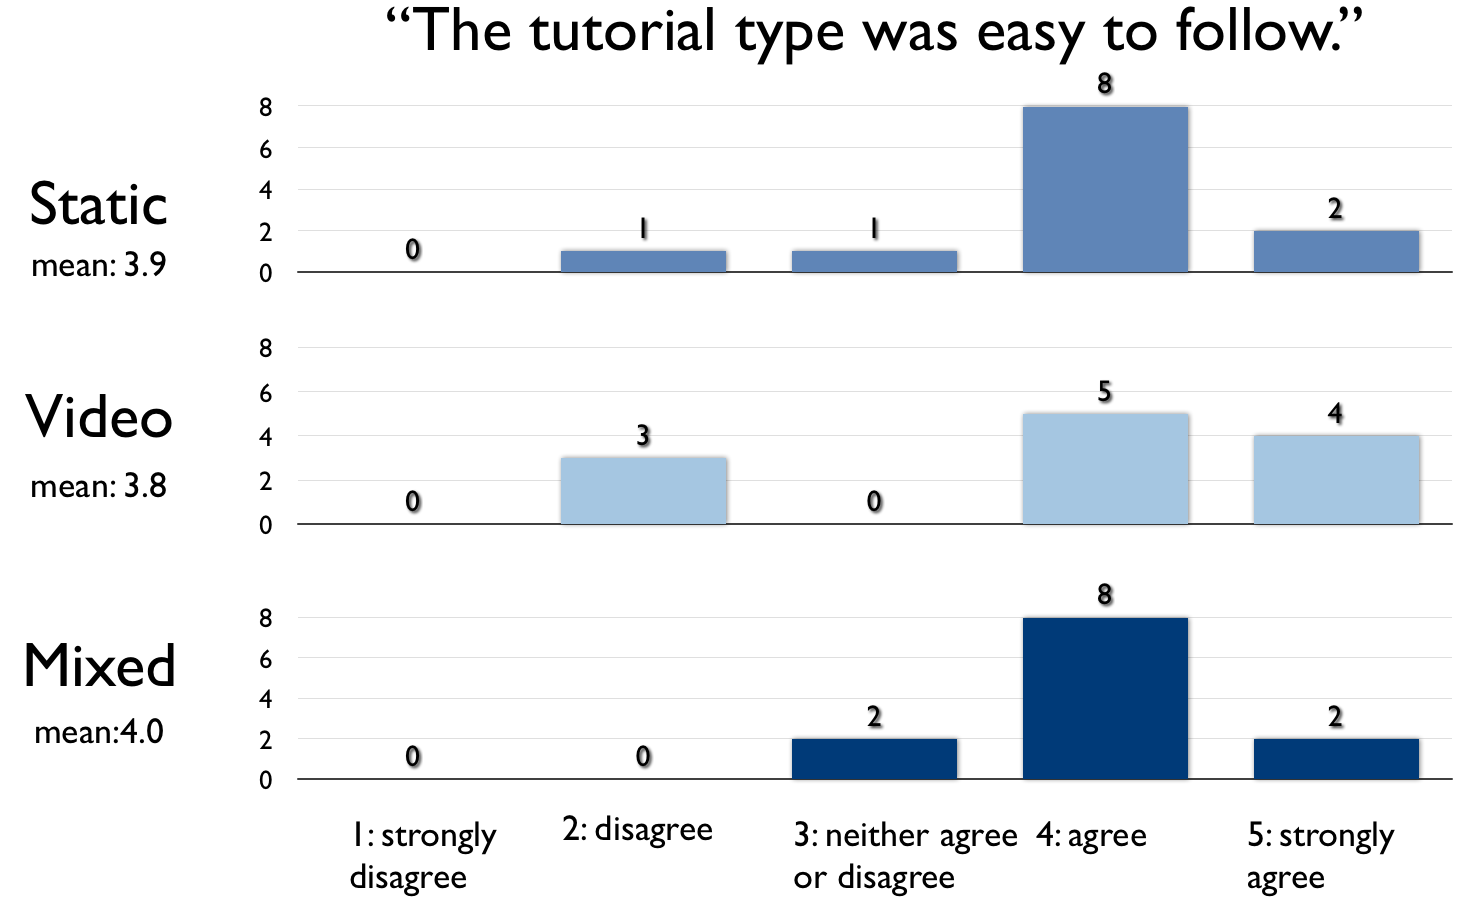
\includegraphics[width=\textwidth]{\demowiz/fig/results/likert}
  \caption{User feedback from questionnaire on the 7-point Likert scale.}
  \label{fig:demowiz_likert}
\end{figure*}

\subsubsection{Visualization as a Supportive Cue}
Participants answered that they were able to understand DemoWiz visualization of input events (µ = 6.0) and found it supportive for their presentations (µ = 6.3). They also commented that the DemoWiz visualization supported the presentation in various aspects: \iquote{the visualization reminds of the order of the content} (P1), \iquote{Really liked the ability to know what was coming up} (P2), \iquote{It provides better insight of the progress of the video} (P6), and \iquote{viz gave me an idea about timing or something I was going to forget to say} (P9).

\subsubsection{Narration Timing}
We coded the 20 recordings of participants' final presentations to observe the timing of narration of each action in correspondence with the video content (11 key events for both tasks). With DemoWiz, participants tended to \textit{anticipate} the upcoming events rather than talk afterwards, where the average timing was -0.1 seconds with DemoWiz (i.e., narrated the action before it happened) and 0.4 seconds with the Baseline condition (i.e., explained the action after it was shown). We found a significant difference in the number of times that events were anticipated by the narration, co-occurred, or occurred after the fact ($\chi $\textsuperscript{2}\textit{(2,220) = 8.6, p = .01}, see Figure~\ref{fig:demowiz_results_timing}).

In general, this supports our suspicion that DemoWiz would help in anticipating an event as opposed to talking about it after it occurred. More important though, was how often a narrator spoke about an event within several seconds of when the event actually occurred. By defining \textit{better} timing as when a presenter's explanation came within 2 seconds of a shown event (either prior, exact, or after), there was marginal significance by condition (\textit{p} = .089 with DemoWiz performing better). In addition, with the Baseline condition, the timing of narration was less consistent and off more, varying from 6 seconds early or 10 seconds late with a variance of 3.9 seconds, in comparison to the DemoWiz condition with at most 3 seconds early to 3 seconds late and a variance of 1.9 seconds.

Five participants had an obvious \textit{error} (forgot the next action or incorrectly narrated another action), had a long \textit{break} (waiting for more than 2 seconds until the action was made), or \textit{missed} an action (did not explain an important feature) when presenting with the Baseline condition. On the other hand, in the DemoWiz condition no errors were made, and there were only one long break and one miss from two different participants, respectively.

Participants' comments also support the fact that DemoWiz helped presenters anticipate the upcoming events. P7 explained, \iquote{(I) felt better able to time my speech to coincide with visual events, rather than trailing after them. Without the event visualizations, I felt like I was talking about what the audience had just seen, rather than having my words and visuals combine to a single message.}

\begin{figure*}[t]
  \centering
  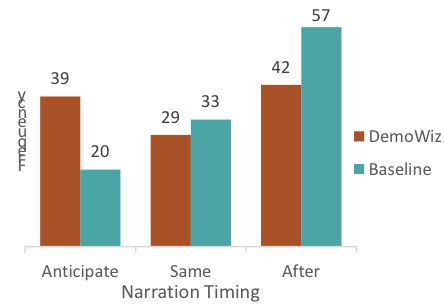
\includegraphics[width=\textwidth]{\demowiz/fig/results_timing}
  \caption{The number of times events were anticipated by the narration, co-occurred, or occurred after the fact.}
  \label{fig:demowiz_results_timing}
\end{figure*}

\subsubsection{Editing Experience}
We collected comments on the workflow. Participants found it easy to record (µ = 6.4) their demonstrations with DemoWiz. For editing features, they found it easy to edit in general (6.6), including controlling the playback speed (6.5) and adding pauses and stops (6.5), but it was less easy to add text notes (4.8); only two participants used this as reminders.

Although using different strategies, all of the participants adjusted the playback speed for matching their narration. Some sped up whenever possible and added stop markers for transitions; some slowed down the repetitive actions (such as drags) to demonstrate effects. P6 said, \iquote{I really liked being able to add ‘stop' events so I could \'fake\' my demo better.} DemoWiz made it easy for participants to separate the capturing and presentation preparation as P5 explained, \iquote{Overall, recording was very easy. In fact, as I got to the second task, I realized that I really don't need to think about the words as I record because later on I will be able to slow down and speed up time ...}

On average, the length of demo videos was 2'09\" before editing and 2'05\" after editing, and the presentation was 2'38\" long. Each participant spent 7.5 minutes on average to edit. For each demo of 44 segments on average, participants adjusted 3.15 segments for speedup and 4.25 segments for slowdown, and added 0.55 pause markers. In the DemoWiz condition, 1.2 stop markers and 0.2 text notes were added.

%!TEX root = ../thesis.tex
\subsection{Results}

\begin{figure*}[!t]
  \centering
  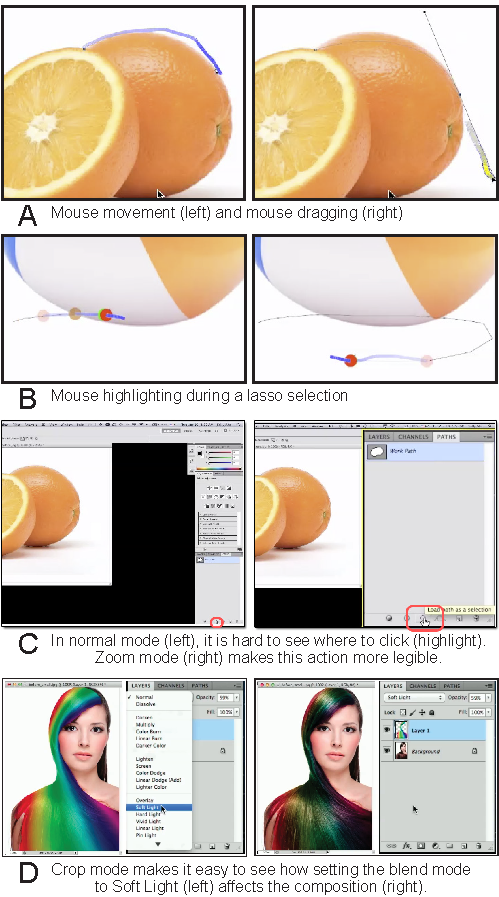
\includegraphics[width=0.95\textwidth]{\mixt/fig/mixt_results/mixt_results}
  \caption{Automatically-generated MixT results.}
  \label{fig:mixt_results}
\end{figure*}

We gathered nine different tutorials and recorded working through each tutorial in Photoshop. We then used MixT to automatically generate mixed media tutorials from these demonstrations. This section describes this corpus. The following section then evaluates the generated tutorials quantitatively and qualitatively.

Our tutorials came from both online and book sources: two from ``Adobe Photoshop CS5 Classroom in a Book,'' five from photoshopstar.com, one from makeuseof.com, and one from icanbecreative.com. All are popular resources for Photoshop learners. Two of the tutorials were also used in the formative user study. The selected tutorials had a total of 165 steps and covered all five command types: they contained 15 brushing/drawing operations, 14 control point manipulations, 30 parameter adjustments, 67 UI navigations, and 39 layer operations. The demonstrations were recorded on three different laptops running Photoshop in full screen with native resolutions of 1680x1050, 1440x900, and 1280x800 pixels.

Overall, the MixT tutorials that we generated exhibit the desired characteristics that we identified in our formative study: scannable steps, small but legible videos, visualized mouse operations, and user control over presentation format. We highlight some interesting results generated by MixT and also refer readers to the provided video figure, which has additional examples.

\subsubTitleBold{Scannability} The step-by-step layout of our tutorials makes them easy to scan. For example, at a glance, we see that the tutorial ``Turning an Image into an Old Photo'' involves several adjustment layer operations, while the tutorial ``Creating Artistic Effects'' involves more parameter adjustments and brushing commands.

\subsubTitleBold{Mouse visualization} Our mouse visualizations help clarify several interactions. They clearly communicate the difference between clicking and dragging, a distinction that is fundamental to operations such as path manipulation but hard to glean from screen capture video. For example, Figure~\ref{fig:mixt_results}A shows the difference between moving around the contour of an object without drawing a path (left), and dragging a Bézier handle to adjust a path segment (right). Mouse trails and click markers were also useful for showing the trajectory of lasso selections (Figure~\ref{fig:mixt_results}B).

\subsubTitleBold{Zoom and crop modes} For many steps, the zoom and crop videos offer clear legibility benefits over the normal video mode. In our corpus, zoom mode was especially valuable for highlighting actions on small buttons that occurred near the frame boundaries, e.g., in the layers palette (Figure~\ref{fig:mixt_results}C right). Such operations are easy to miss in a normal, scaled video (Figure~\ref{fig:mixt_results}C left). Crop mode was useful in showing the effect that parameter selection has on the canvas. Figure~\ref{fig:mixt_results}D shows two successive frames that illustrate how changing a layer's blending mode affects the image. Enlarging the canvas in these modes also helps users see the details of effects, such as applying the eraser tool on the canvas to enhance the underlying layer (Figure~\ref{fig:mixt_mouse}).



%!TEX root = ../thesis.tex
\section{Conclusion}

In this chapter, we presented DemoCut, a semi-automatic video editing
system that helps users create clear and concise video tutorials of
DIY tasks. The key idea behind our approach is to combine rough user
annotations with simple video and audio analysis techniques in order
to segment the input recording and apply appropriate editing
effects. Our small user evaluation suggests that video authors are
able to create effective video tutorials using DemoCut, and the
qualitative feedback includes encouraging positive reactions to the
annotation and editing workflow, as well as the automatic editing
effects.

% \section{Limitations and Future Work}

Our implementation is based on several simplifying assumptions that
limit generality. We assume a single, static camera position that
shows all relevant actions and a quiet indoor environment with
constant lighting and little background noise. In order to detect static shots  that should be skipped, our video analysis assumes a static background. Our audio analysis assumes that all non-silent sections of audio are narration, but this may not always be the case. Loud non-speech sounds, such as chopping or the sound of a sewing machine, can lead to errors in our editing effect decisions.

As was pointed out by several of our study participants, making effect decisions individually for each segment can lead to inconsistencies in playback speed as the video transitions from segment to segment. A more global approach that looks at all video effects together and enforces  smooth transitions between adjacent segments would help address some of these artifacts.
%
In addition to addressing these limitations, we see several promising
directions for future work.

\subsubTitleBold{Multiple camera footage.} We designed DemoCut to work with
footage from a single, static camera. One interesting avenue for
future work is to consider footage from multiple cameras. Prior work has compared different camera views capturing physical
tasks for remote collaboration \cite{Fussell:2003te,Ranjan:2007}. Similarly, DemoCut could try to automatically select the best view for
each segment based on user annotations as well as the video content
(e.g., choosing a zoomed view for closeups, switching to a
different view when there are occlusions). % \bh{cite Ranjan here?}

\subsubTitleBold{Support viewer's learning.} In this work, we focus on producing
well-edited video tutorials. However, we could also imagine generating
different output formats, including indexed
videos, step-by-step instructions, or mixed media tutorials, similar
to those presented by Chi et al.~\cite{Chi:2012:MAG:2380116.2380130}. Another natural extension would
be to develop interactive components that monitor user actions and
provide realtime guidance and feedback for general DIY tasks. Follow-up studies to understand viewer's learning experience would be useful for refining the automatic editing effects and interactive design.
% Different output formats and understand viewer's perspective.
% {\bf Interactive DIY tutorials.} Recent work has demonstrated
% interactive tutorial systems that help users follow specific types of
% physical tasks, such as assembling Duplo models~\cite{Gupta:2012ku}.
% A natural extension of our work would
% be to develop interactive components that monitor user actions and
% provide realtime guidance and feedback for general DIY tasks.

\subsubTitleBold{Generalize to other instructional video domains.} One exciting direction is to explore other areas where our techniques could be applied, such as software learning, music instruction, and video lectures. Each domain may require slightly different analysis and segmentation rules. For example, the system could use a log of executed operations to adjust segment boundaries for software tutorials, or incorporate pitch detection when analyzing music instruction.

% \section{Acknowledgments}

% Work at Berkeley was supported by Adobe and a Berkeley Fellowship for Graduate Studies.
% %
% We thank the YouTube users (in alphabetical order) \textit{donyboy73, Griffin Hammond on Indy Mogul, John NYCCNC, Matt Richardson on MAKE, mjfpieters, and TheMuskokaPainter} for sharing their insights on DIY tutorials in our interviews.

%\bh{still need to fix widows and orphans throughout.}

